% Opcje klasy 'iithesis' opisane sa w komentarzach w pliku klasy. Za ich pomoca
% ustawia sie przede wszystkim jezyk oraz rodzaj (lic/inz/mgr) pracy.
\documentclass[inz, shortabstract]{iithesis}

\usepackage[utf8]{inputenc}
\usepackage{graphicx}


%%%%% DANE DO STRONY TYTUŁOWEJ
% Niezaleznie od jezyka pracy wybranego w opcjach klasy, tytul i streszczenie
% pracy nalezy podac zarowno w jezyku polskim, jak i angielskim.
% Pamietaj o madrym (zgodnym z logicznym rozbiorem zdania oraz estetyka) recznym
% zlamaniu wierszy w temacie pracy, zwlaszcza tego w jezyku pracy. Uzyj do tego
% polecenia \fmlinebreak.
\polishtitle    {Aplikacja pomagająca użytkownikom \fmlinebreak zrozumieć swoje emocje oraz identyfikować \fmlinebreak wzorce nastroju}
\englishtitle   {A mobile application helping users understand their emotions and \fmlinebreak identify mood patterns}
\polishabstract {Celem pracy jest stworzenie aplikacji mobilnej, która umożliwi użytkownikom identyfikowanie własnych emocji oraz czynników wpływających na ich występowanie. 
Aplikacja ma ułatwić rozpoznawanie źródeł stresu oraz wspierać podejmowanie decyzji promujących zdrowsze nawyki. Dzięki wykorzystaniu identyfikacji wpływu czynników tj. dieta, aktywność fizyczna i sen na nastrój użytkownik zostaje stopniowo uświadomiony o powiązaniu jego stylu życia ze zdrowiem psychicznym. Zadaniem aplikacji jest również proponowanie wskazówek na podstawie emocji odczuwanych przez użytkownika, jak i zapewnienie możliwości swobodnego opisywania codziennych przemyśleń czy doświadczeń.}
\englishabstract{The goal of the thesis is to create a mobile application that allows users to identify their own emotions and the factors that influence them. 
The app is intended to facilitate the identification of sources of stress and support decision-making that promotes healthier habits. By identifying the influence of factors such as diet, physical activity and sleep on mood, the user will gradually become aware of the link between their lifestyle and mental health. The app is also designed to provide guidance based on the user's emotions, as well as the ability to freely describe daily thoughts or experiences.}
% w pracach wielu autorow nazwiska mozna oddzielic poleceniem \and
\author         {Aleksandra Nicpoń \and Martyna Wybraniec}
% w przypadku kilku promotorow, lub koniecznosci podania ich afiliacji, linie
% w ponizszym poleceniu mozna zlamac poleceniem \fmlinebreak
\advisor        {dr Marcin Młotkowski}
%\date          {}                     % Data zlozenia pracy
% Dane do oswiadczenia o autorskim wykonaniu
%\transcriptnum {}                     % Numer indeksu
%\advisorgen    {dr. Jana Kowalskiego} % Nazwisko promotora w dopelniaczu
%%%%%

%%%%% WLASNE DODATKOWE PAKIETY
%
%\usepackage{graphicx,listings,amsmath,amssymb,amsthm,amsfonts,tikz}
%
%%%%% WŁASNE DEFINICJE I POLECENIA
%
%\theoremstyle{definition} \newtheorem{definition}{Definition}[chapter]
%\theoremstyle{remark} \newtheorem{remark}[definition]{Observation}
%\theoremstyle{plain} \newtheorem{theorem}[definition]{Theorem}
%\theoremstyle{plain} \newtheorem{lemma}[definition]{Lemma}
%\renewcommand \qedsymbol {\ensuremath{\square}}
% ...
%%%%%

\begin{document}

%%%%% POCZĄTEK ZASADNICZEGO TEKSTU PRACY

\chapter{Wprowadzenie}
W dzisiejszych czasach dbanie o własne zdrowie psychiczne jest niezwykle ważne. Ilość informacji, jakie na co dzień przetwarzamy, powoduje, że stajemy się przebodźcowani i często nie zdajemy sobie sprawy, jak intensywnie oddziałuje to na nasze samopoczucie. Zarówno życie zawodowe, jak i nawet prywatne często zmusza nas do ukrywania emocji, maskowania ich lub ignorowania na potrzeby zachowania pozorów. Z tego powodu postanowiłyśmy stworzyć narzędzie, które pomoże nam nie tylko zidentyfikować ukrywające się emocje, ale również znaleźć powiązania między nimi a czynnościami wykonanymi przez nas danego dnia.

Nasza aplikacja ma służyć jako asystent do samorefleksji. Jej głównym zadaniem jest subtelne nakierowanie użytkownika do wyciągnięcia wniosków na temat swojego stanu psychicznego. Aby to osiągnąć, musimy przede wszystkim zachować równowagę pomiędzy zapewnieniem swobody w wyborze emocji a odpowiednim ograniczaniem pola wyboru na rzecz ułatwienia użytkownikowi procesu analizy.

\chapter{Przypadki użycia}

Każdy scenariusz rozpoczyna się uruchomieniem aplikacji przez użytkownika.
\section{Analiza samopoczucia}
\begin{enumerate}
	\item Użytkownik loguje się do aplikacji.
	\item Użytkownik znajduje się na głównej stronie.
	\item Aplikacja wita użytkownika oraz pyta się o jego samopoczucie.
	\item Użytkownik naciska przycisk \textit{Let's find out together!}.
	\item Aplikacja przekierowuje użytkownika do ekranu wyboru stopnia \textit{przyjemności} odczuwanych emocji.
	\item Użytkownik za pomocą suwaka wybiera stopień oraz naciska przycisk \textit{next}.
	\item Aplikacja przekierowuje użytkownika do ekranu wyboru stopnia \textit{energii} odczuwanych emocji.
	\item Użytkownik za pomocą suwaka wybiera stopień oraz naciska przycisk \textit{next}.
	\item Aplikacja wyświetla emocje o podobnym stopniu przyjemności i energii.
	\item Użytkownik zaznacza emocje najlepiej opisujące jego samopoczucie.
	\item Aplikacja zapisuje wybór użytkownika i przekierowuje go do ekranu ankiety dotyczącej czynników wpływających na samopoczucie.
	\item Użytkownik odpowiednio wybiera długość swojego snu, natężenie aktywności fizycznej, posiłki spożyte danego dnia oraz czynności, jakie wykonał (praca, szkoła, relaks).
	\item Dodany wpis jest teraz widoczny na stronie głównej.
\end{enumerate}

\section{Przeglądanie widoku kalendarza}
\begin{enumerate}
	\item Użytkownik loguje się do aplikacji.
	\item Użytkownik znajduje się na głównej stronie.
	\item Użytkownik naciska na ikonę kalendarza na pasku nawigacyjnym.
	\item Aplikacja przekierowuje użytkownika do widoku kalendarza.
	\item Użytkownik przegląda miesięczny kalendarz z kolorystycznymi wskazówkami odpowiadającymi samopoczuciu zapisanym danego dnia.
	\item Użytkownik wybiera jeden z pokolorowanych dni.
	\item Aplikacja wyświetla użytkownikowi informacje dotyczące emocji oraz parametrów zaznaczonych tego dnia (sen, aktywność fizyczna, ilość spożytych posiłków).
\end{enumerate}

\section{Przeglądanie statystyk}
\begin{enumerate}
	\item Użytkownik loguje się do aplikacji.
	\item Użytkownik znajduje się na głównej stronie.
	\item Użytkownik naciska na ikonę wykresu na pasku nawigacyjnym.
	\item Aplikacja przekierowuje użytkownika do widoku statystyk.
	\item Użytkownik przegląda wykresy przedstawiające rozkład jego emocji zapisanych w ostatnim tygodniu, miesiącu, oraz raporty analityczne przedstawiające powiązania między emocjami a parametrami takimi jak sen czy aktywność fizyczna.
\end{enumerate}

\section{Dodawanie wpisu do dziennika}
\begin{enumerate}
	\item Użytkownik loguje się do aplikacji.
	\item Użytkownik znajduje się na głównej stronie.
	\item Użytkownik naciska na pole tekstowe zatytułowane \textit{Something on your mind?}
	\item Aplikacja przekierowuje użytkownika do widoku tworzenia wpisu w dzienniku.
	\item Użytkownik opisuje swoje doświadczenia, myśli, lub wydarzenia z dnia.
	\item Użytkownik naciska przycisk \textit{save}.
	\item Aplikacja zapisuje wpis oraz wyświetla go na stronie głównej.
\end{enumerate}



\chapter{Opis i analiza zagadnienia}
\section{Identyfikacja emocji}
Najbardziej popularną metodą opisywania emocji w ogólnodostępnych aplikacjach zwanych \textit{mood trackerami} jest skala emotikonowa. Jest to zwykle pięć ikonek przedstawiających podstawowe wyrazy twarzy kojarzone z negatywnymi, neutralnymi lub pozytywnymi emocjami - płacz, smutek, brak emocji, lekki uśmiech, szeroki uśmiech. Taka skala jest wystarczająca dla osób, które nie odczuwają potrzeby głębszej analizy swojego samopoczucia. Osoby pragnące dowiedzieć się więcej o sobie oraz przeprowadzić bardziej szczegółową identyfikację własnych uczuć nie będą usatysfakcjonowane takim podejściem. 

Z tego powodu postanowiłyśmy użyć bardziej precyzyjnego, dwuwymiarowego modelu emocji stworzonego przez Jamesa A. Russela (1980). \textit{The Valence-Arousal Model} to kołowy diagram składający się z dwóch osi: walencji oraz pobudzenia. Russel pokazał, że każdą emocję można opisać za pomocą tych dwóch zmiennych i odpowiednio umieścić ją na diagramie. Idea ta została później rozwinięta przez psychologa Marca A. Bracketta z Yale Center of Emotional Intelligence i opisana w jego książce \textit{Permission To Feel}.


Korzystając z wyżej wymienionych idei, listy emocji sporządzonej przez \textit{Berkeley Wellbeing Institute}\protect\footnotemark\footnotetext{https://www.berkeleywellbeing.com/list-of-emotions.html} i listy uczuć, emocji i nastrojów autorstwa \textit{Jody Michael Associates}\protect\footnotemark, stworzyłyśmy bazę 256 emocji z przypisanymi krótkimi definicjami oraz współrzędnymi \textit{pleasantness} (przyjemność) i \textit{energy} (energia). Korzystając z tej bazy, będziemy w stanie proponować emocje najbardziej zbliżone do położenia stanu emocjonalnego użytkownika na układzie \textit{Valence-Arousal}.


\footnotetext{https://www.jodymichael.com/blog/jma-feelings-list/}

\begin{figure}[!ht]
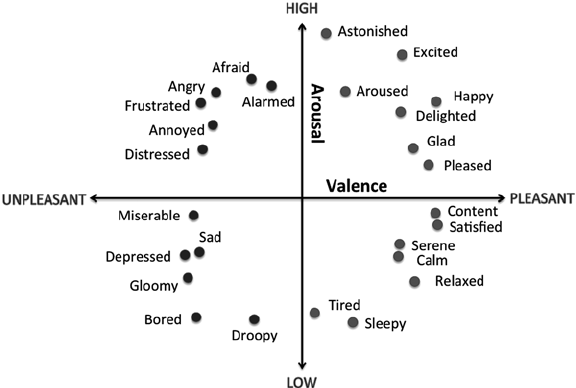
\includegraphics[width=1\textwidth]{Russells-Valence-Arousal-Model.png} 
\caption{\textit{The Valence-Arousal Model} opracowany przez Jamesa A. Russela.\protect\footnotemark}
\end{figure}
\footnotetext{https://www.researchgate.net/figure/Two-dimensional-model-of-valence-and-arousal-adapted-from-Russell-1980\_fig1\_278783929}


\begin{figure}[!hb]
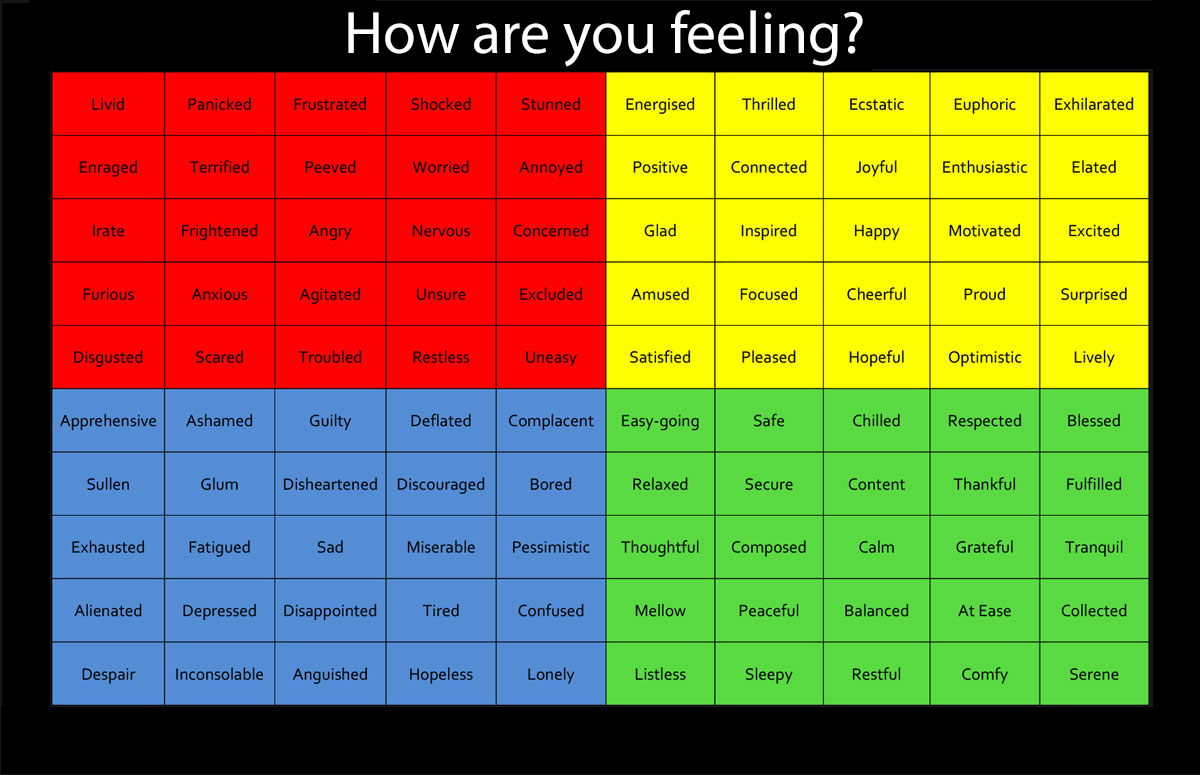
\includegraphics[width=1\textwidth]{mood-meter.jpg} 
\caption{\textit{The Mood Meter} opracowany przez Marca A. Bracketta.\protect\footnotemark}
\end{figure}
\footnotetext{https://www.accelerateco.com/blogs/news/ignite-your-leadership-potential-emotional-literacy-your-secret-weapon-for-high-performing-teams}


\section{Generowanie wykresów i raportów analitycznych}
Kolejnym kluczowym elementem naszej aplikacji jest generowanie statystyk dotyczących nastroju oraz stylu życia użytkownika. Chciałyśmy uwzględnić nie tylko podgląd podsumowania emocji z minionego dnia lub tygodnia, ale również np. wpływ intensywności aktywności fizycznej na samopoczucie. Liczba emocji dostępnych w naszej bazie danych sprawiła, że generowane raporty były zbyt skomplikowane i nieczytelne.

Zdecydowałyśmy się więc pogrupować emocje według ich przynależności do odpowiedniej ćwiartki układu współrzędnych i przypisać każdej z nich kolor. Pozwoliło nam to stworzyć przejrzyste wykresy przedstawiające proporcje emocji znajdujących się w poszczególnych ćwiartkach dla każdego przedziału (dla aktywności fizycznej: brak, niska intensywność, średnia intensywność, wysoka intensywność). 

\section{Pobieranie informacji o czynnikach wpływających na nastrój}
Na potrzeby wcześniej wymienionych statystyk musiałyśmy w procesie identyfikacji emocji uwzględnić ankietę na temat podstawowych czynności, w jakich użytkownik brał udział danego dnia. Ważne było to, aby ankieta nie była zbyt długa lub skomplikowana, co zniechęcałoby do jej wypełniania. Ograniczyłyśmy się zatem do czterech zapytań: pytanie o długość snu, spożyte posiłki, intensywność aktywności fizycznej oraz wykonane czynności (odpoczynek, praca, szkoła itp.). 

Początkowo miałyśmy zamiar udostępnić też opcję dodawania własnych czynników, ale wiązało się to ze znacznym przekształcaniem sposobu generowania wykresów, na co nie wystarczyło nam czasu. Uważamy jednak, że te podstawowe opcje w zupełności wystarczą do przeprowadzenia adekwatnej analizy powiązania nawyków z odczuwanymi emocjami.

\chapter{Porównanie konkurencyjnych aplikacji}
Aplikacje do zarządzania czy identyfikacji swojego samopoczucia (ang. \textit{mood trackers}) cieszą się coraz większą popularnością, zatem nie brakuje ich zarówno w Sklepie Google Play (Android), jak i w App Store (iOS). Z uwagi na ilość i różnorodność takich aplikacji przedstawimy cztery najpopularniejsze z nich: \textit{Daylio}, \textit{Moodpress}, \textit{DailyBean} oraz \textit{How We Feel}. Jeśli aplikacja oferuje wersję premium, pod uwagę będziemy brać tylko funkcje dostępne w wersji bezpłatnej.
\section{Daylio}
Metodą kategoryzowania samopoczucia w aplikacji \textit{Daylio} jest wspomniany przez nas wcześniej model emotikonowy składający się z pięciu stopni (Rys. 4.1). Nie pozwala to na głębszą analizę nastroju, lecz wydaje się być idealne dla młodszych użytkowników. 

Po wybraniu samopoczucia aplikacja prosi o zaznaczenie wykonanych tego dnia czynności, opisanie jakości snu czy intensywności aktywności fizycznej. Jest to funkcja niezbędna do wyliczenia statystyk i wykresów (Rys. 4.2), więc uwzględnimy ją również w naszym rozwiązaniu. Standardowo mamy też dostęp do widoku kalendarza, który przedstawia wizualną reprezentację nastrojów logowanych danego miesiąca.


\begin{figure}[!ht]
\centering
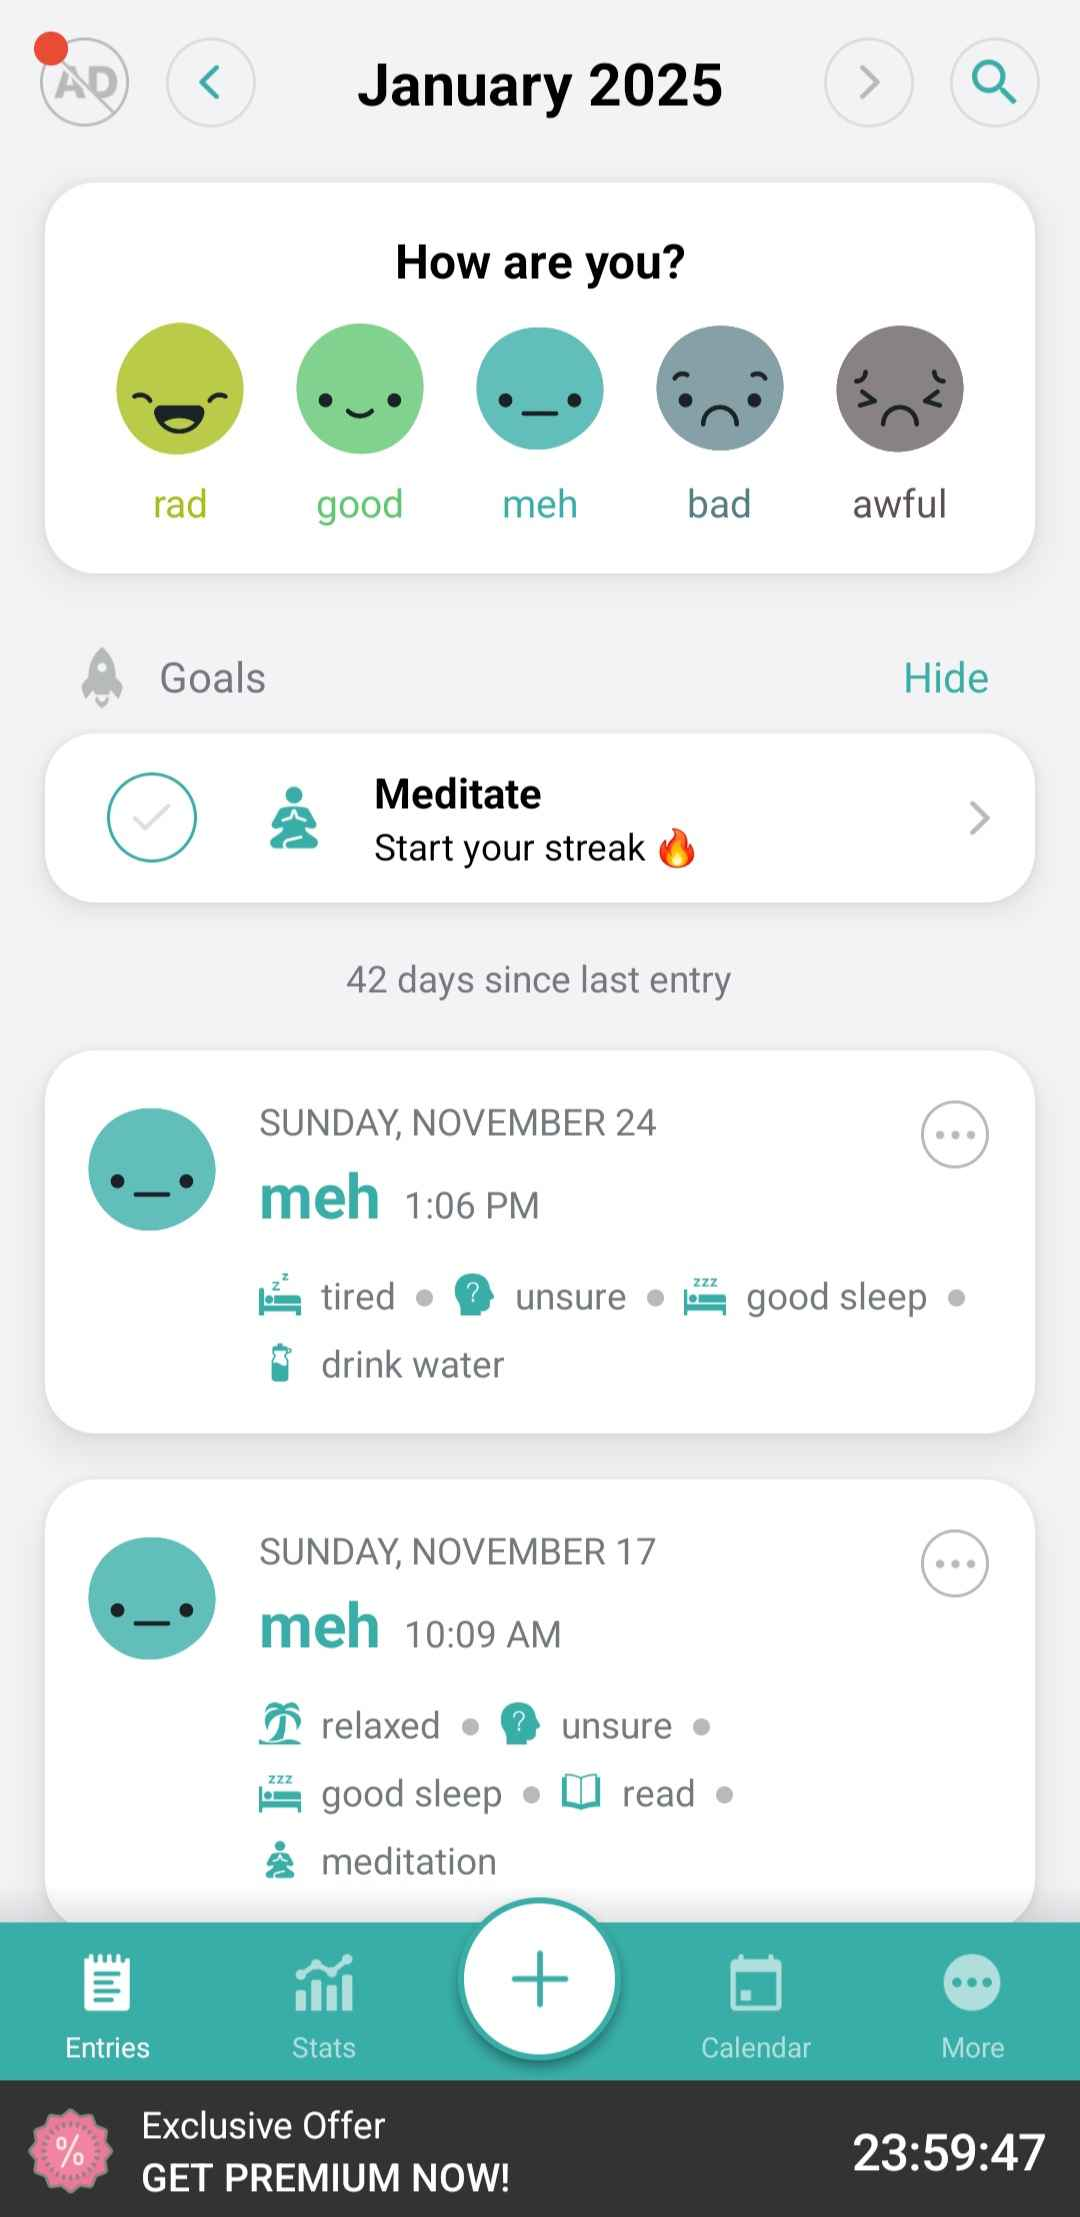
\includegraphics[width=0.35\textwidth]{daylio1.jpg} 
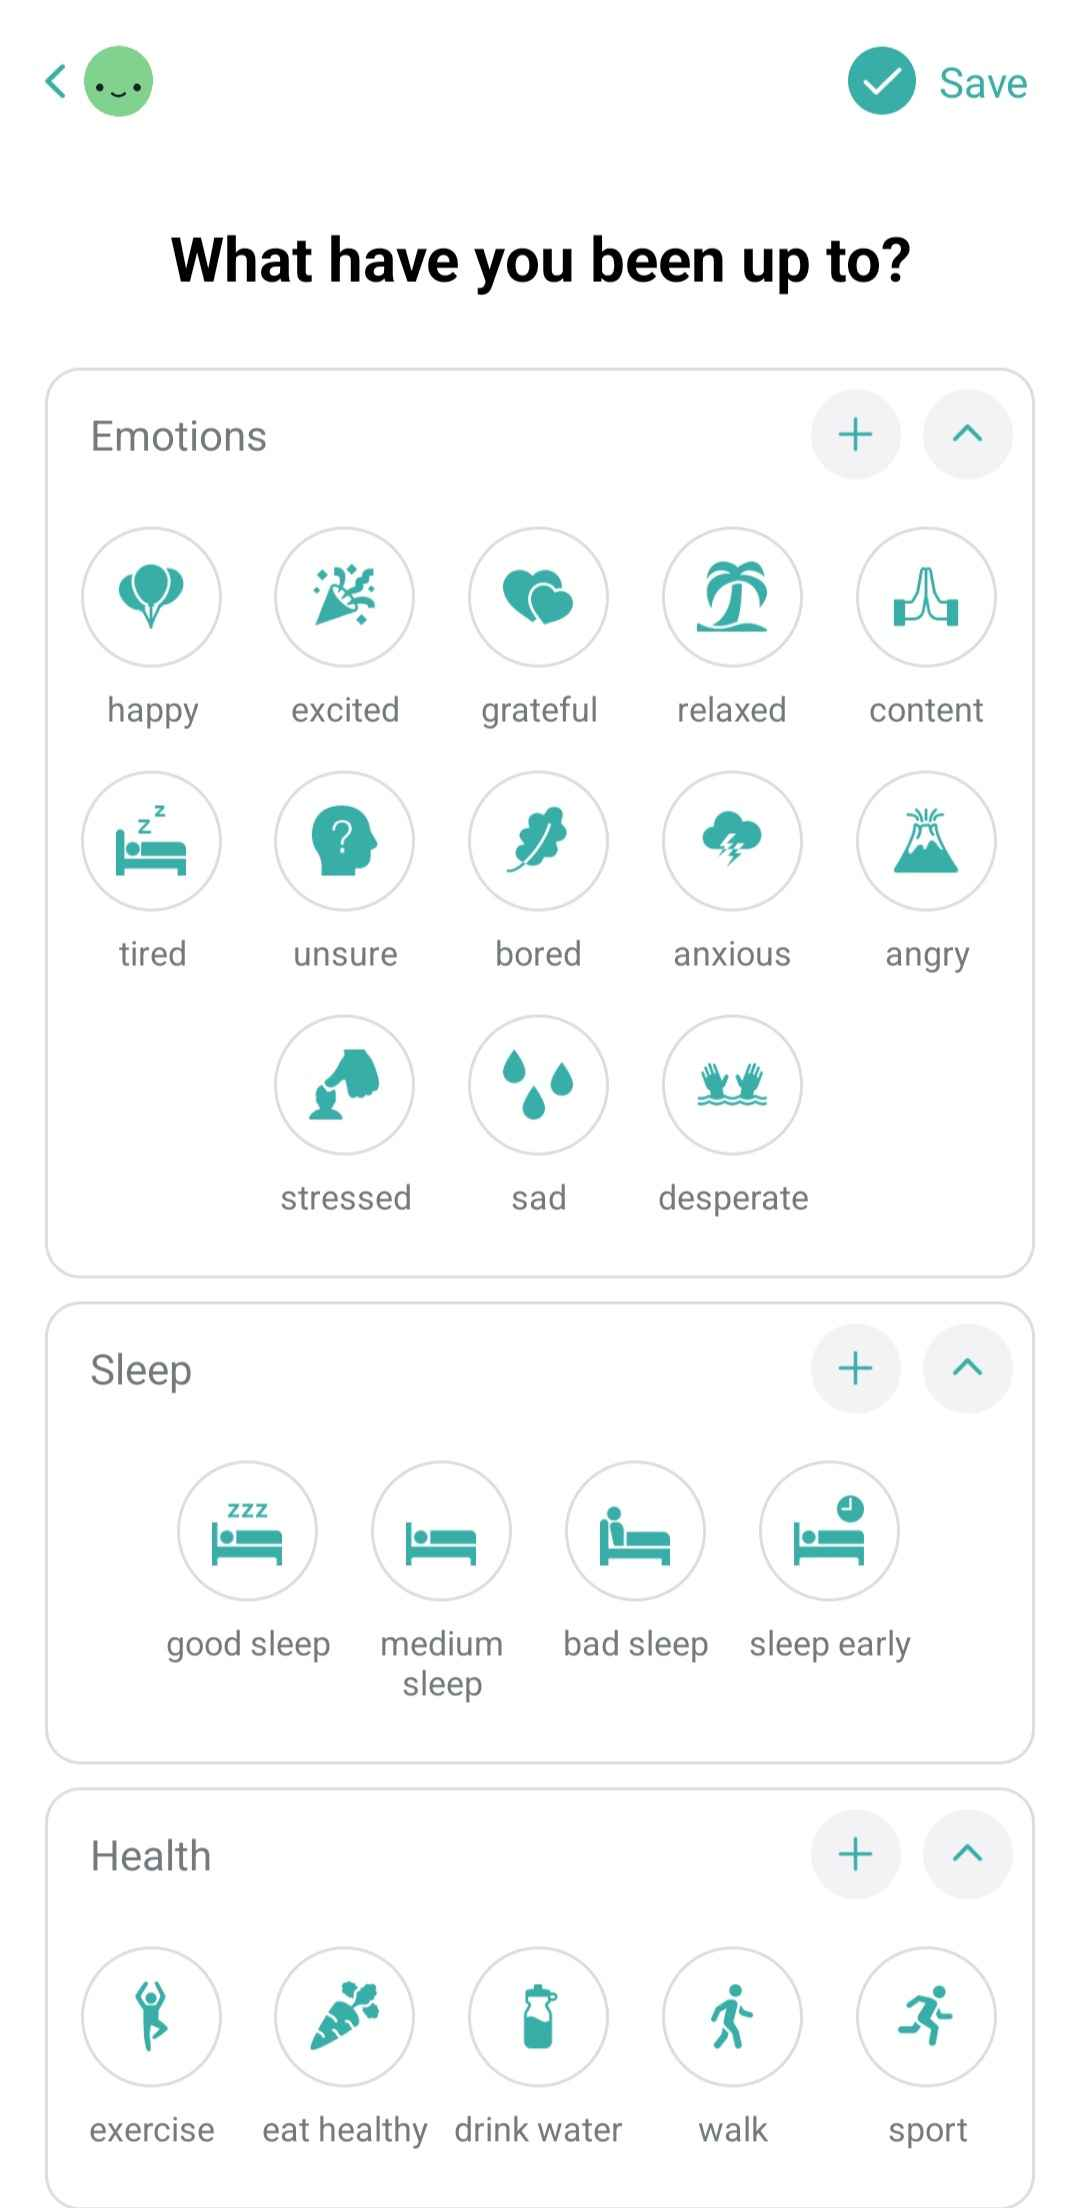
\includegraphics[width=0.35\textwidth]{daylio2.jpg} 
\caption{Widoki wyboru samopoczucia oraz czynników w aplikacji \textit{Daylio}.}
\end{figure}
\begin{figure}[!hb]
\centering
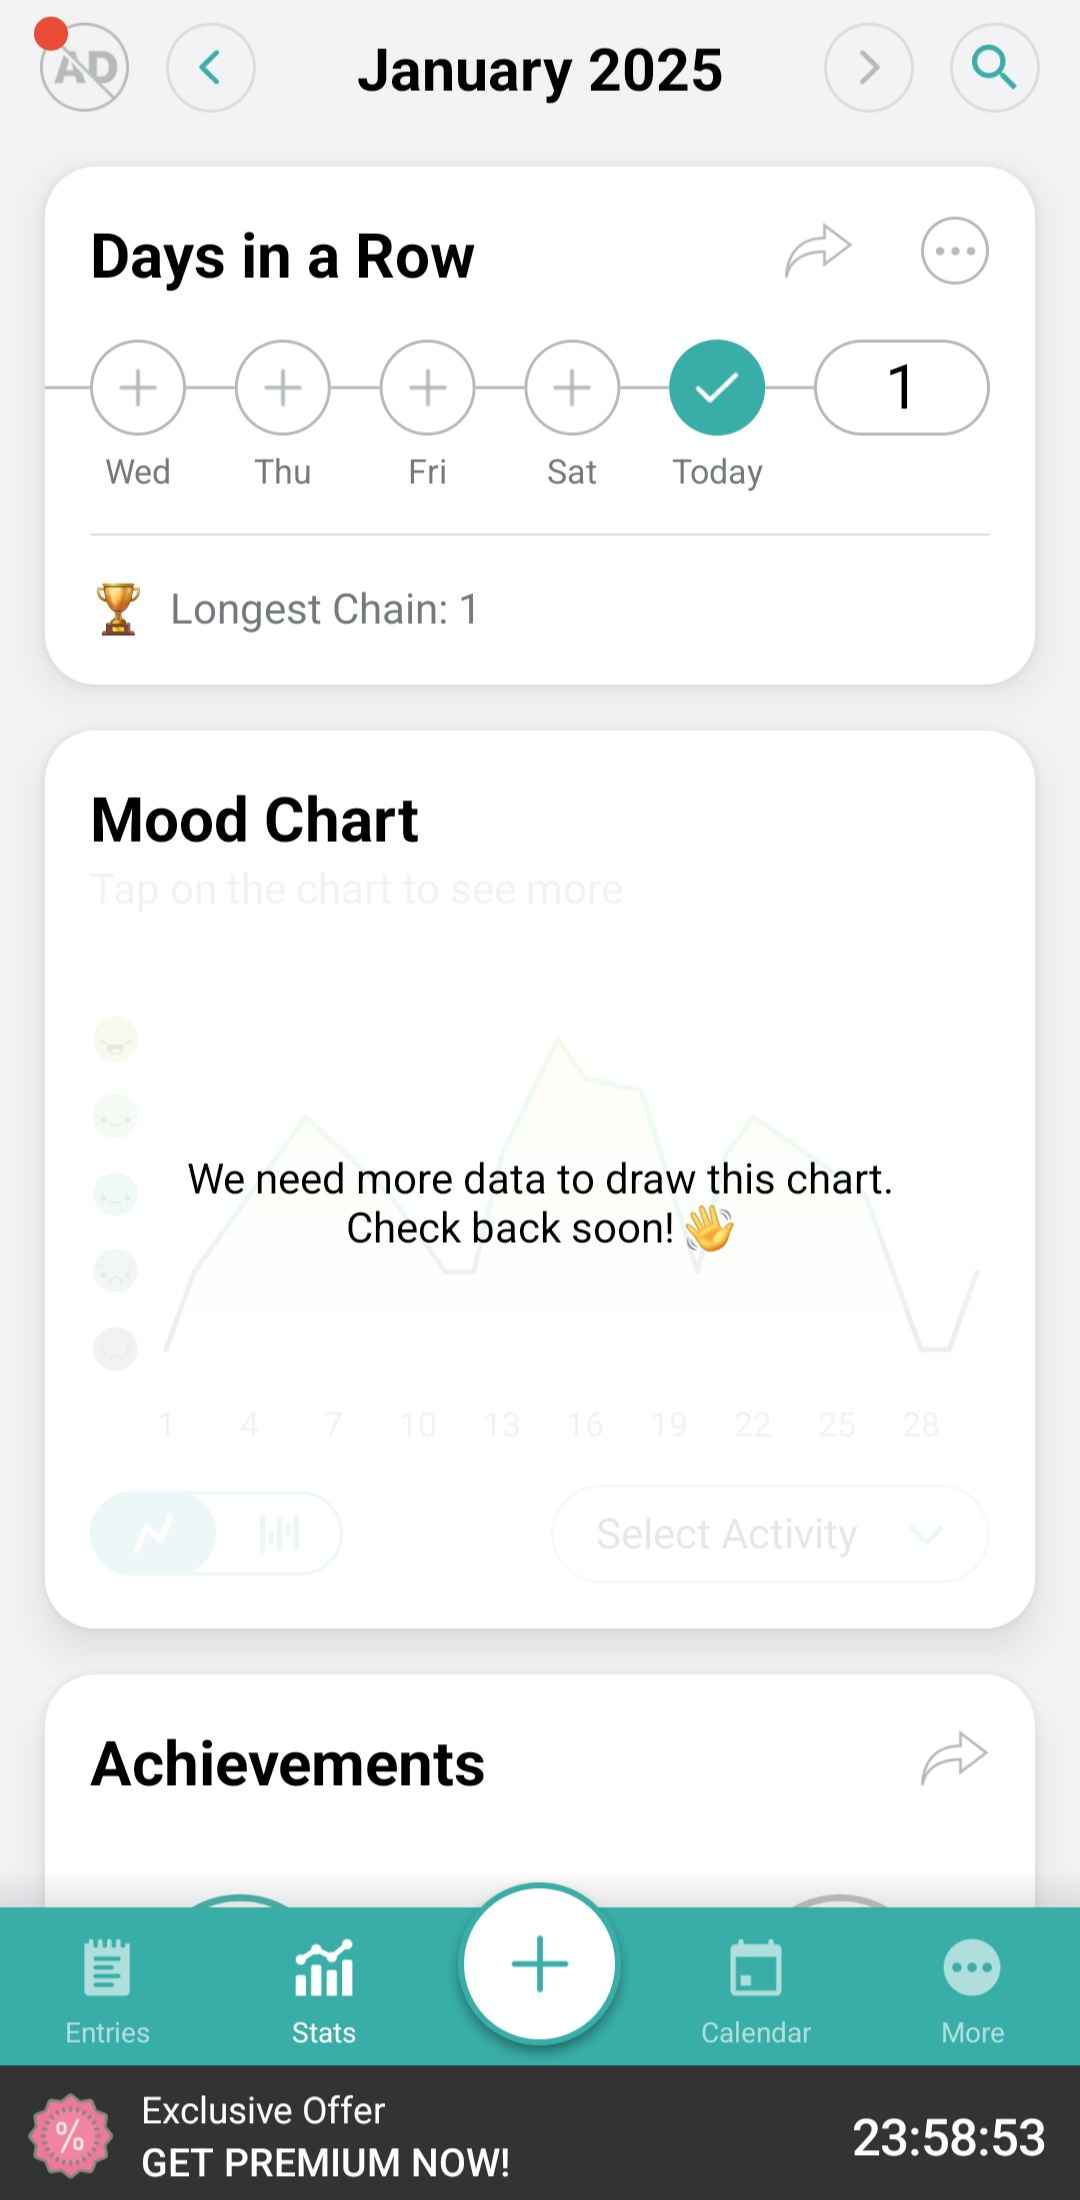
\includegraphics[width=0.35\textwidth]{daylio3.jpg} 
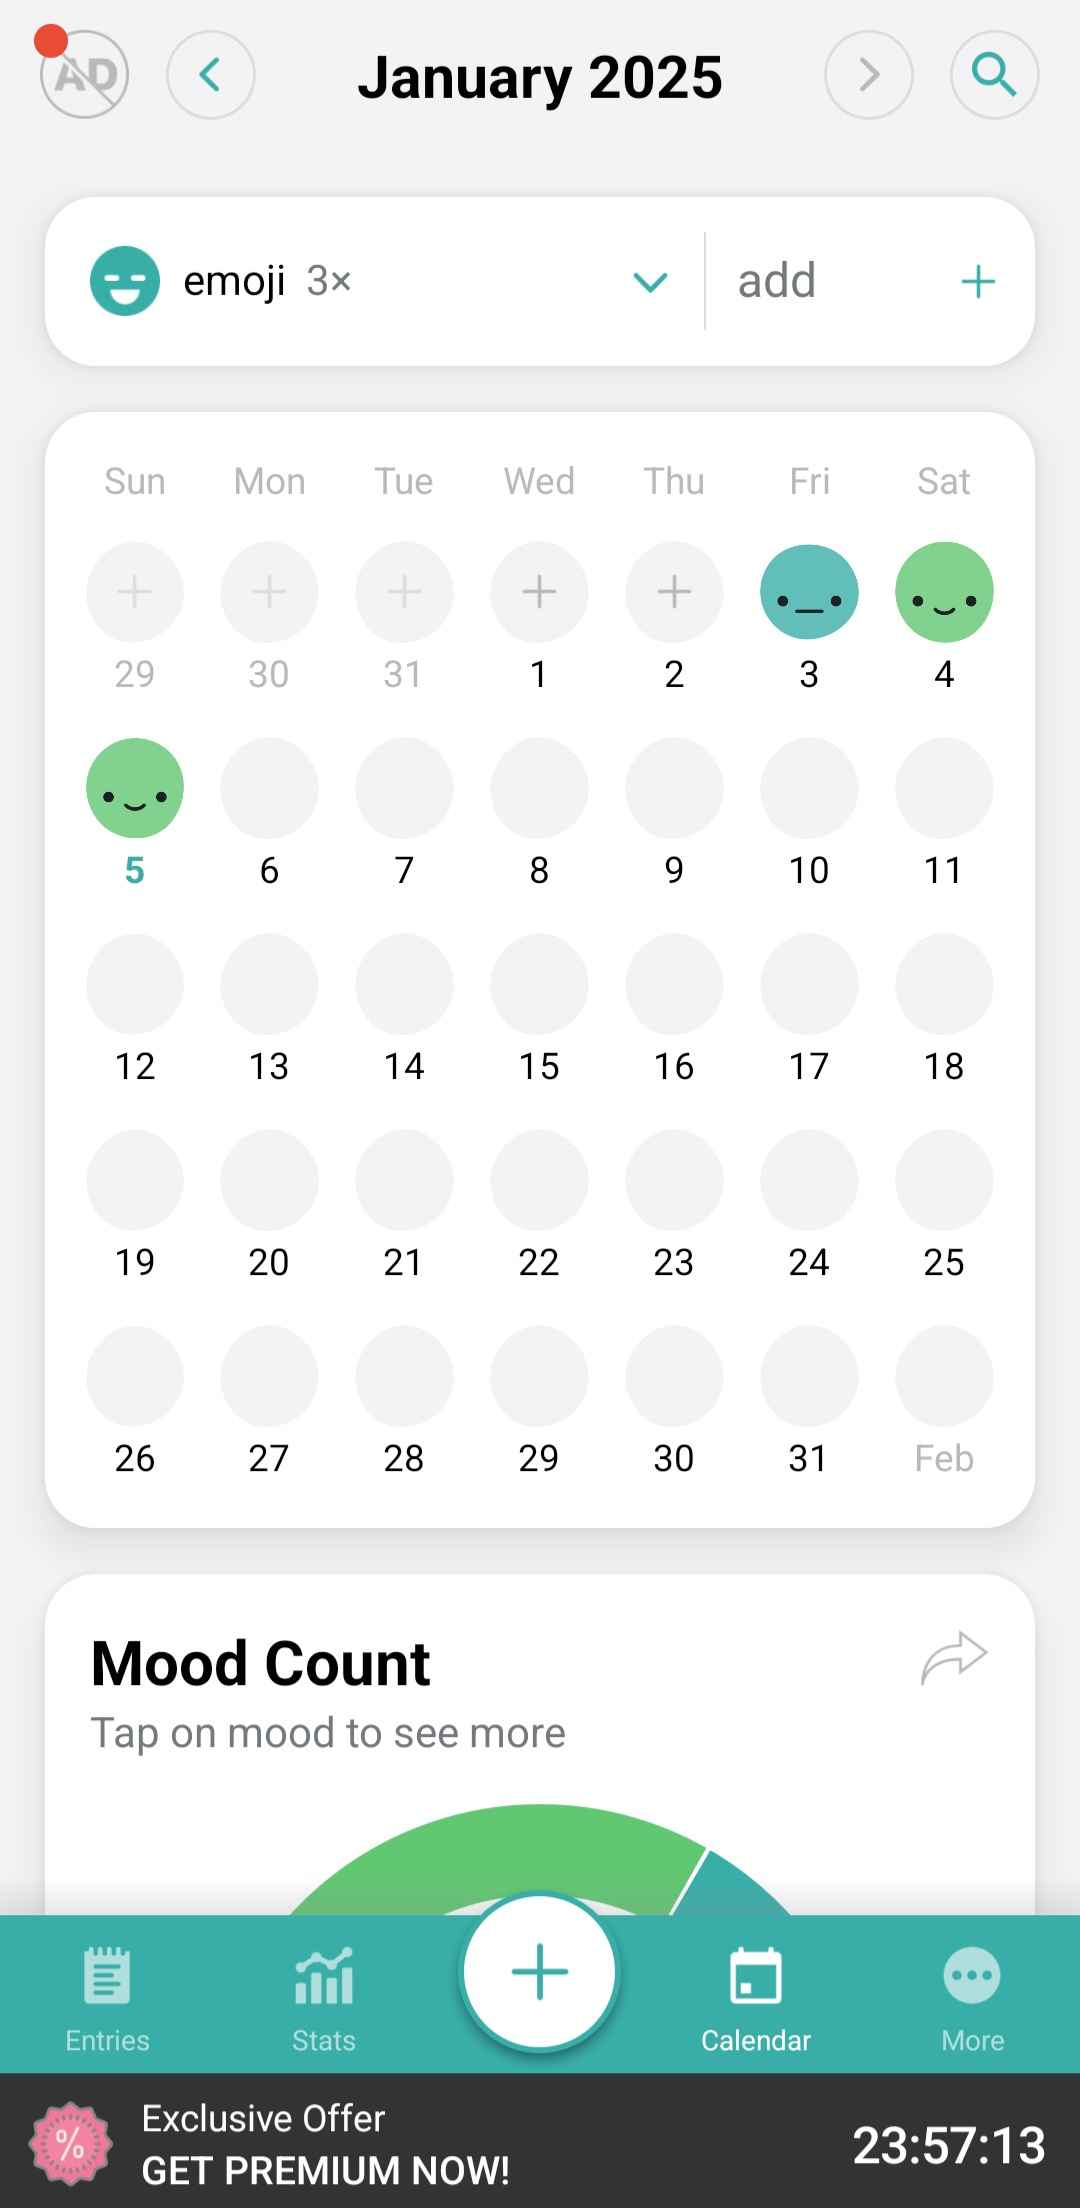
\includegraphics[width=0.35\textwidth]{daylio4.jpg} 
\caption{Widoki statystyk oraz kalendarza w aplikacji \textit{Daylio}.}
\end{figure}

\section{Moodpress}
Aplikacja \textit{Moodpress}, podobnie jak \textit{Daylio}, używa emotikonów do reprezentacji emocji. W tym przypadku jest to okrąg jedenastu ikonek różniących się mimiką twarzy oraz kolorystyką. Daje to większe pole wyboru, jednak nadal ogranicza użytkownika. Emotikony nie są też do końca jednoznaczne, a czasem wręcz nieczytelne, co może utrudnić użytkownikowi prawidłową identyfikację emocji. Brakuje tutaj też możliwości zapisywania czynników wpływających na emocje, jest jednak dostęp do podstawowych statystyk oraz widoku kalendarza.

\begin{figure}[!ht]
\centering
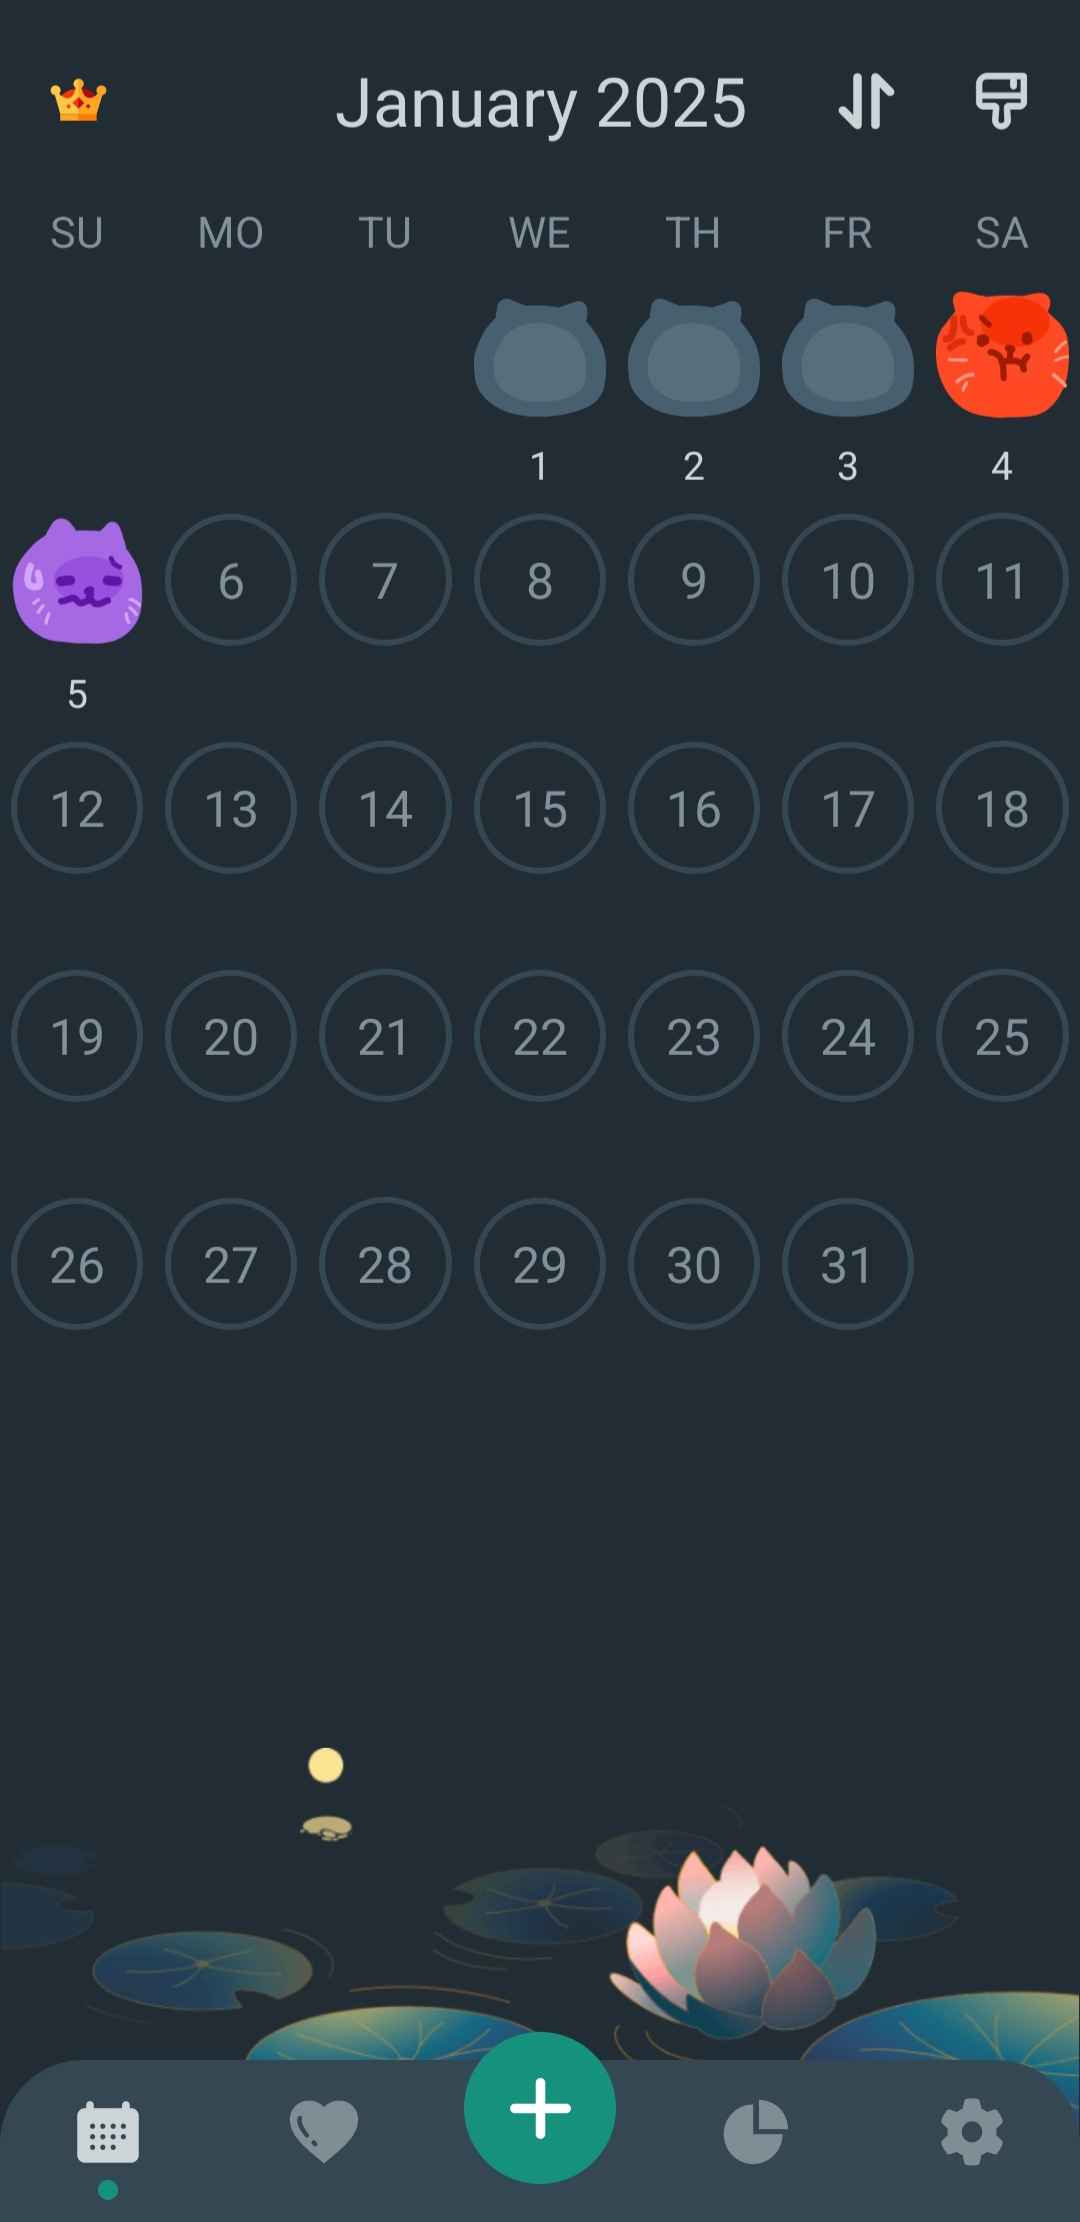
\includegraphics[width=0.3\textwidth]{moodpress1.jpg} 
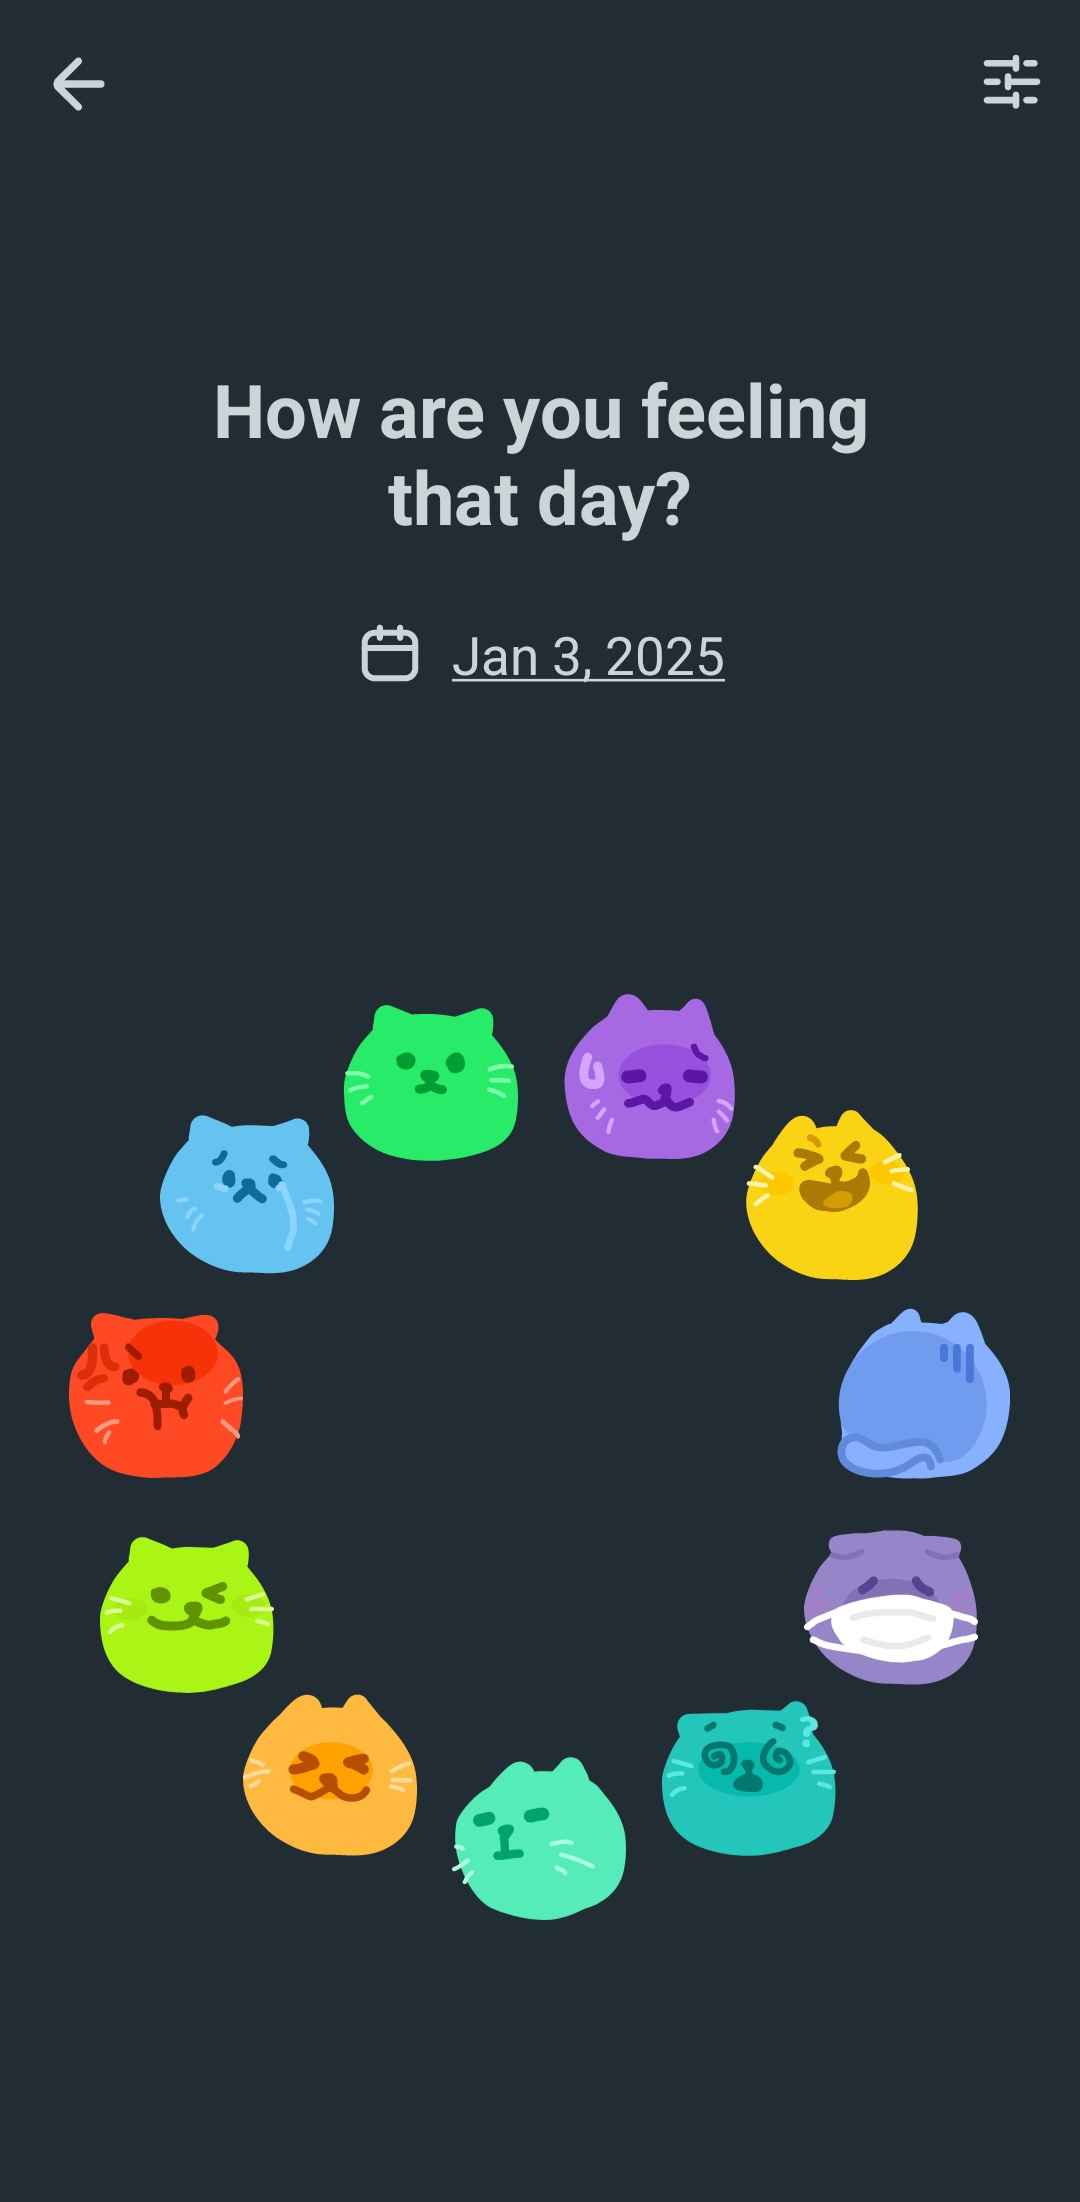
\includegraphics[width=0.3\textwidth]{moodpress2.jpg} 
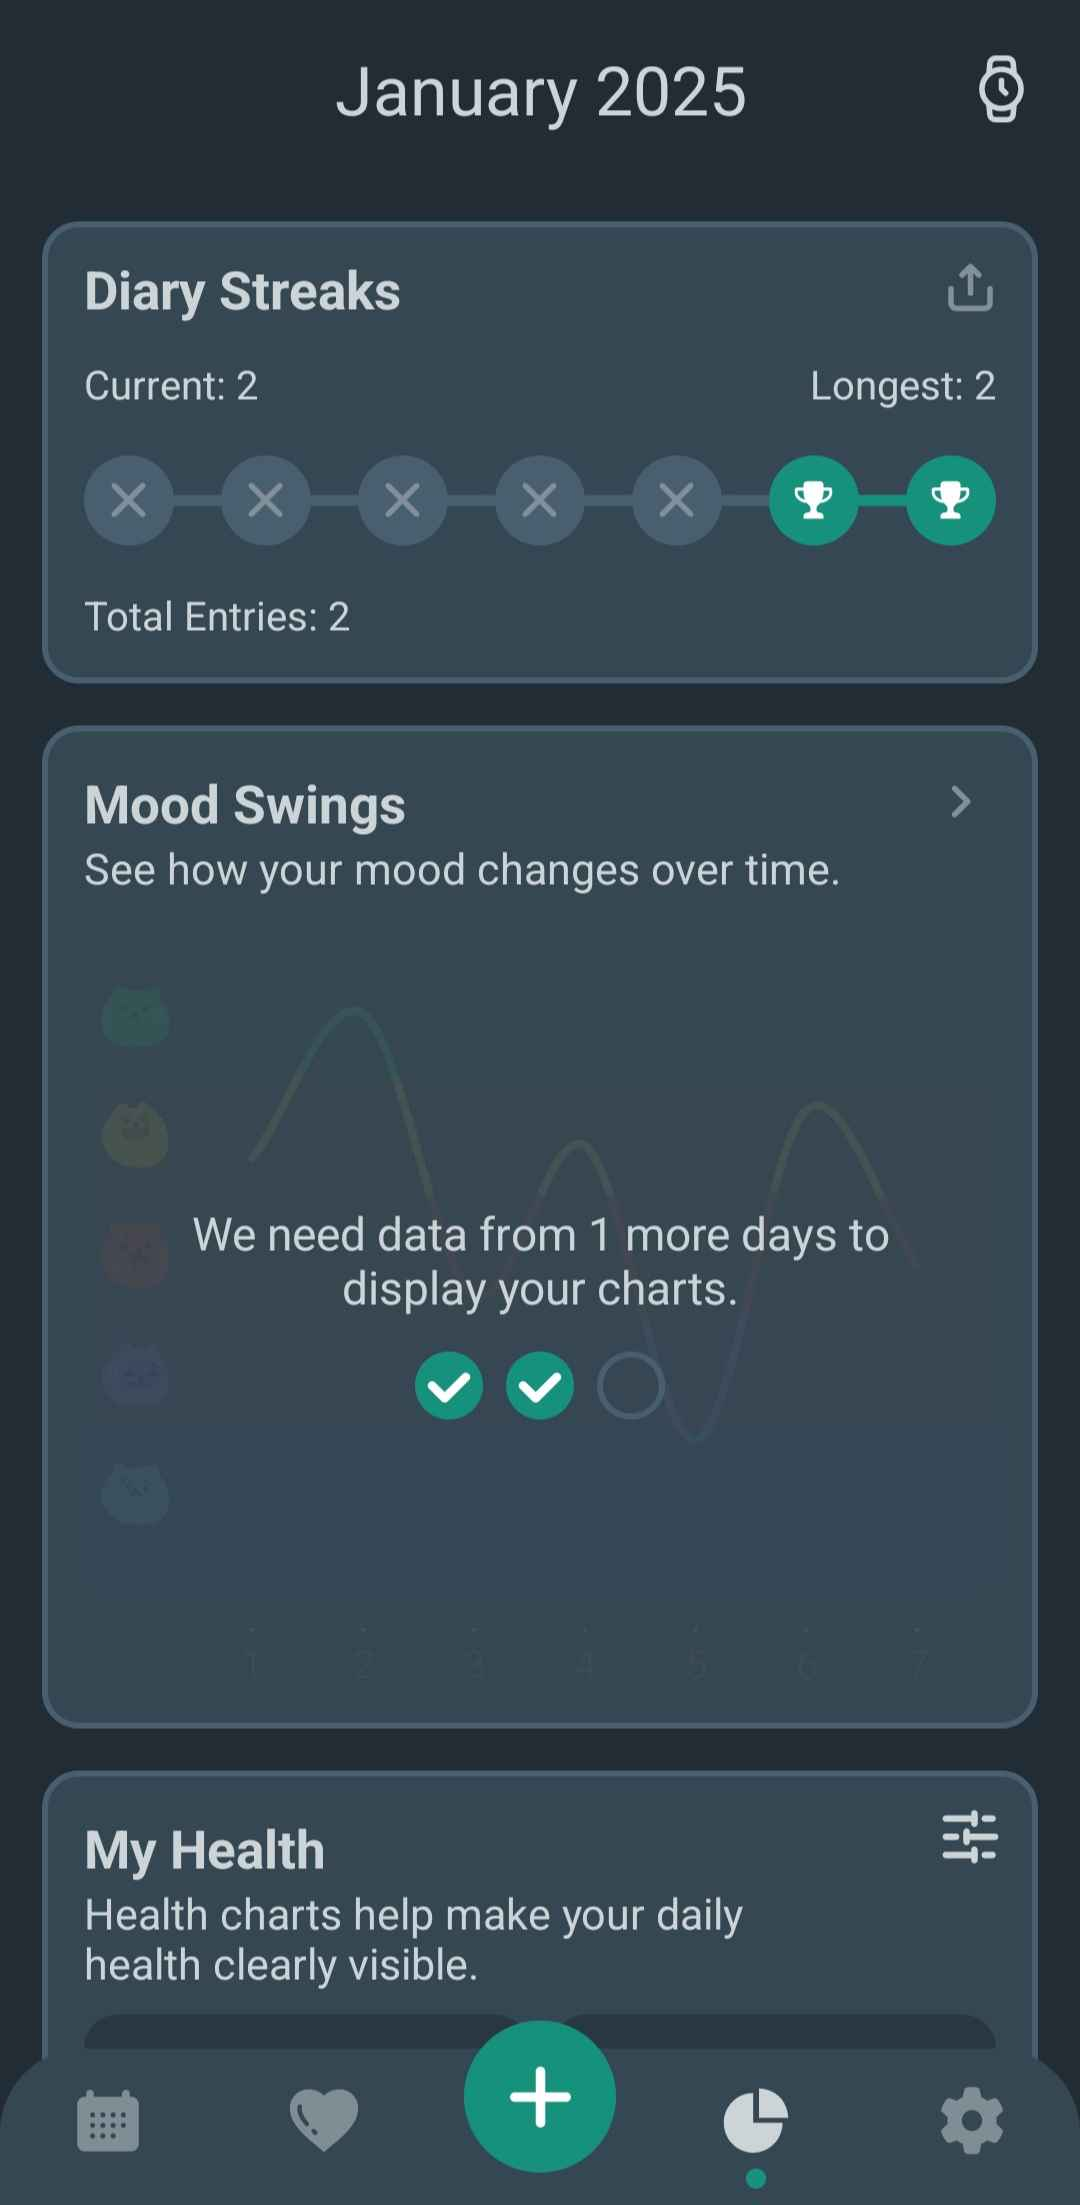
\includegraphics[width=0.3\textwidth]{moodpress3.jpg} 
\caption{Główne widoki aplikacji \textit{Moodpress}.}
\end{figure}

\section{DailyBean}
Trzecim narzędziem do analizy samopoczucia jest \textit{DailyBean}. Na pozór wydaje się być prawie nierozróżnialne od poprzednich dwóch przykładów, jednak oprócz standardowego spektrum emotikonowego jako pierwsze daje użytkownikowi możliwość wyboru spośród dwudziestu emocji (Rys 4.4). Pozwala też na zaznaczenie czynników z wyjątkowo dużej liczby kategorii. Minusem aplikacji jest pojawiający się w wielu miejscach \textit{paywall}, czyli ograniczenie dla użytkowników nieposiadających wersji płatnej (Rys 4.5). 

\begin{figure}[!ht]
\centering
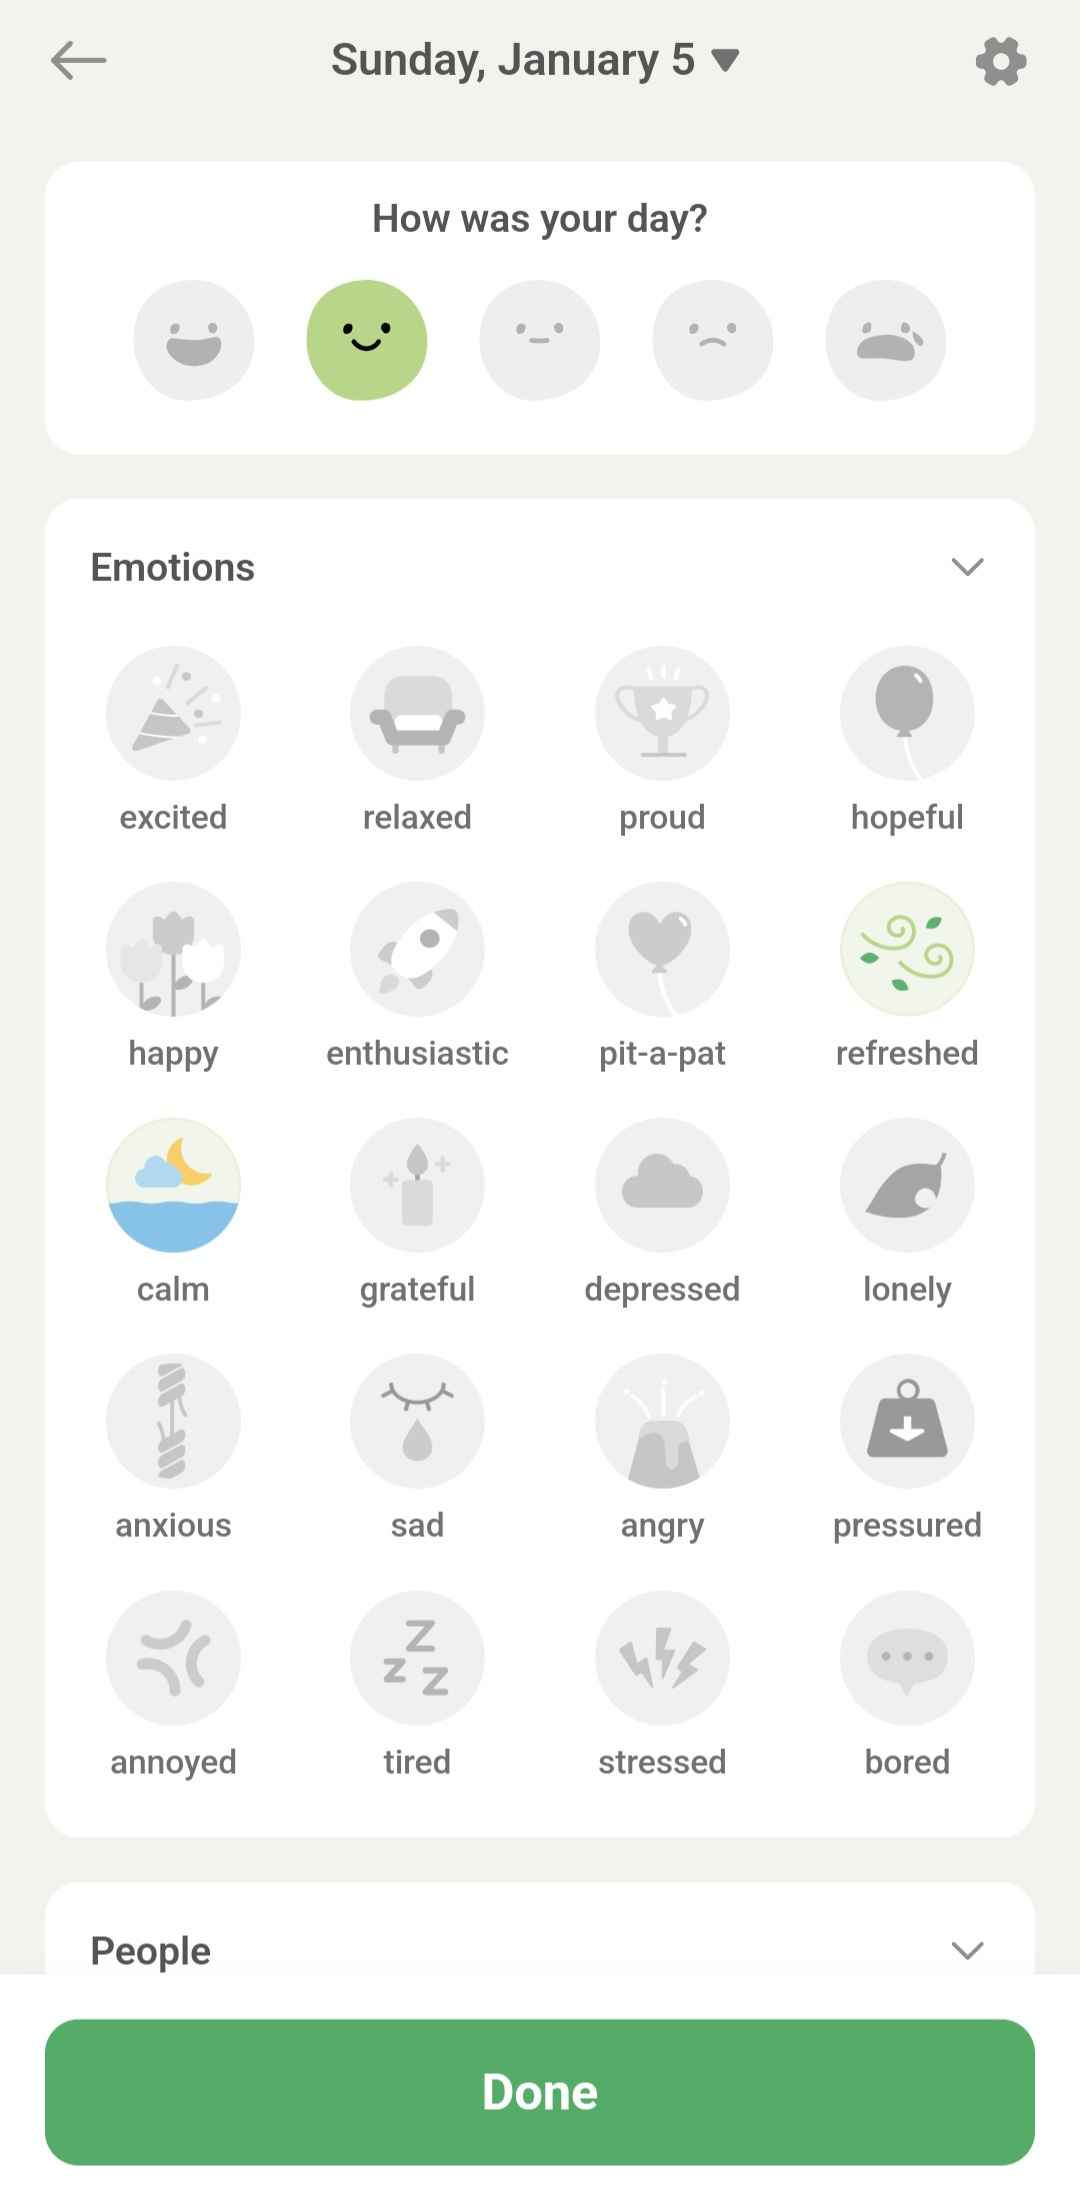
\includegraphics[width=0.35\textwidth]{dailybean1.jpg} 
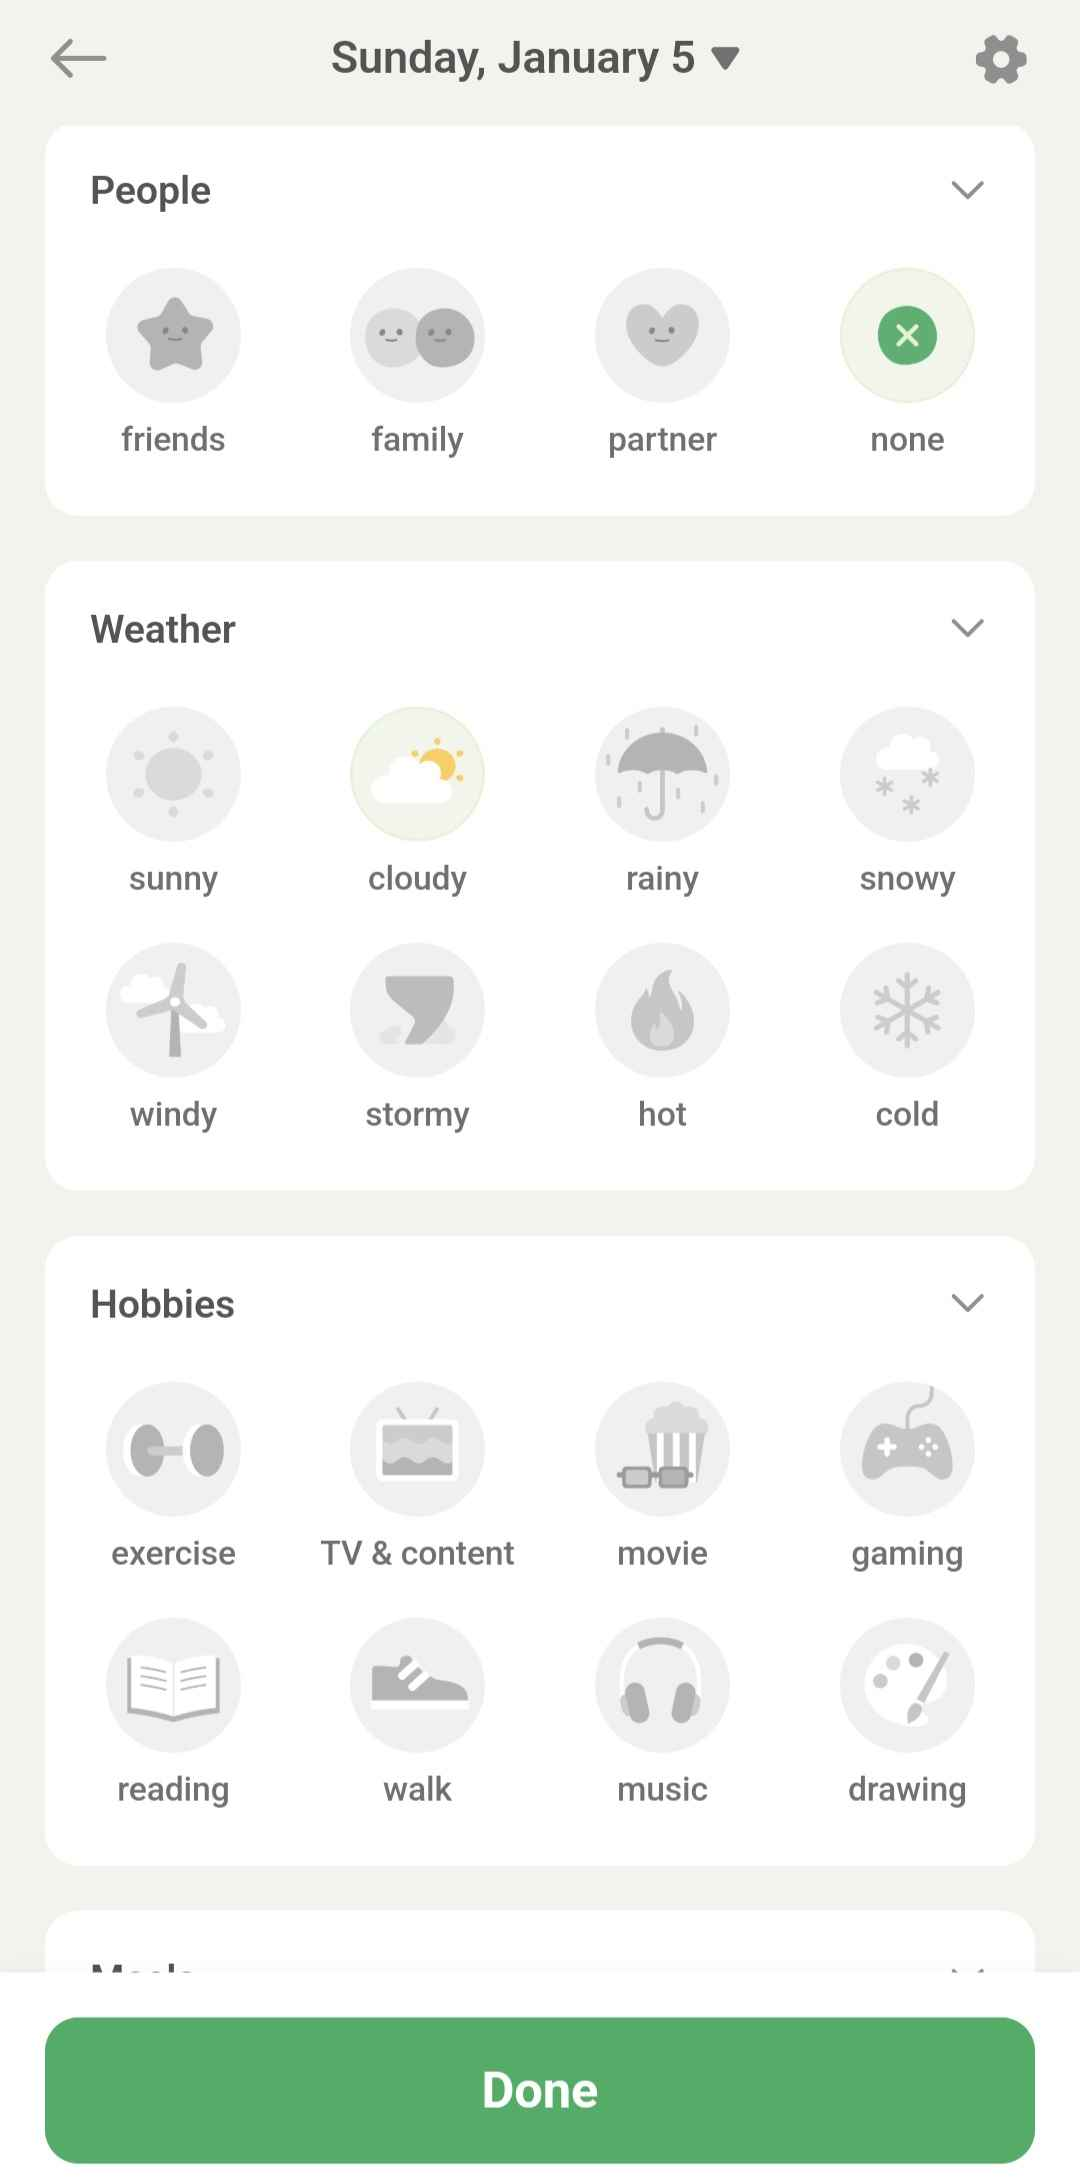
\includegraphics[width=0.35\textwidth]{dailybean2.jpg} 
\caption{Widoki logowania samopoczucia aplikacji \textit{DailyBean}.}
\end{figure}

\begin{figure}[!hb]
\centering
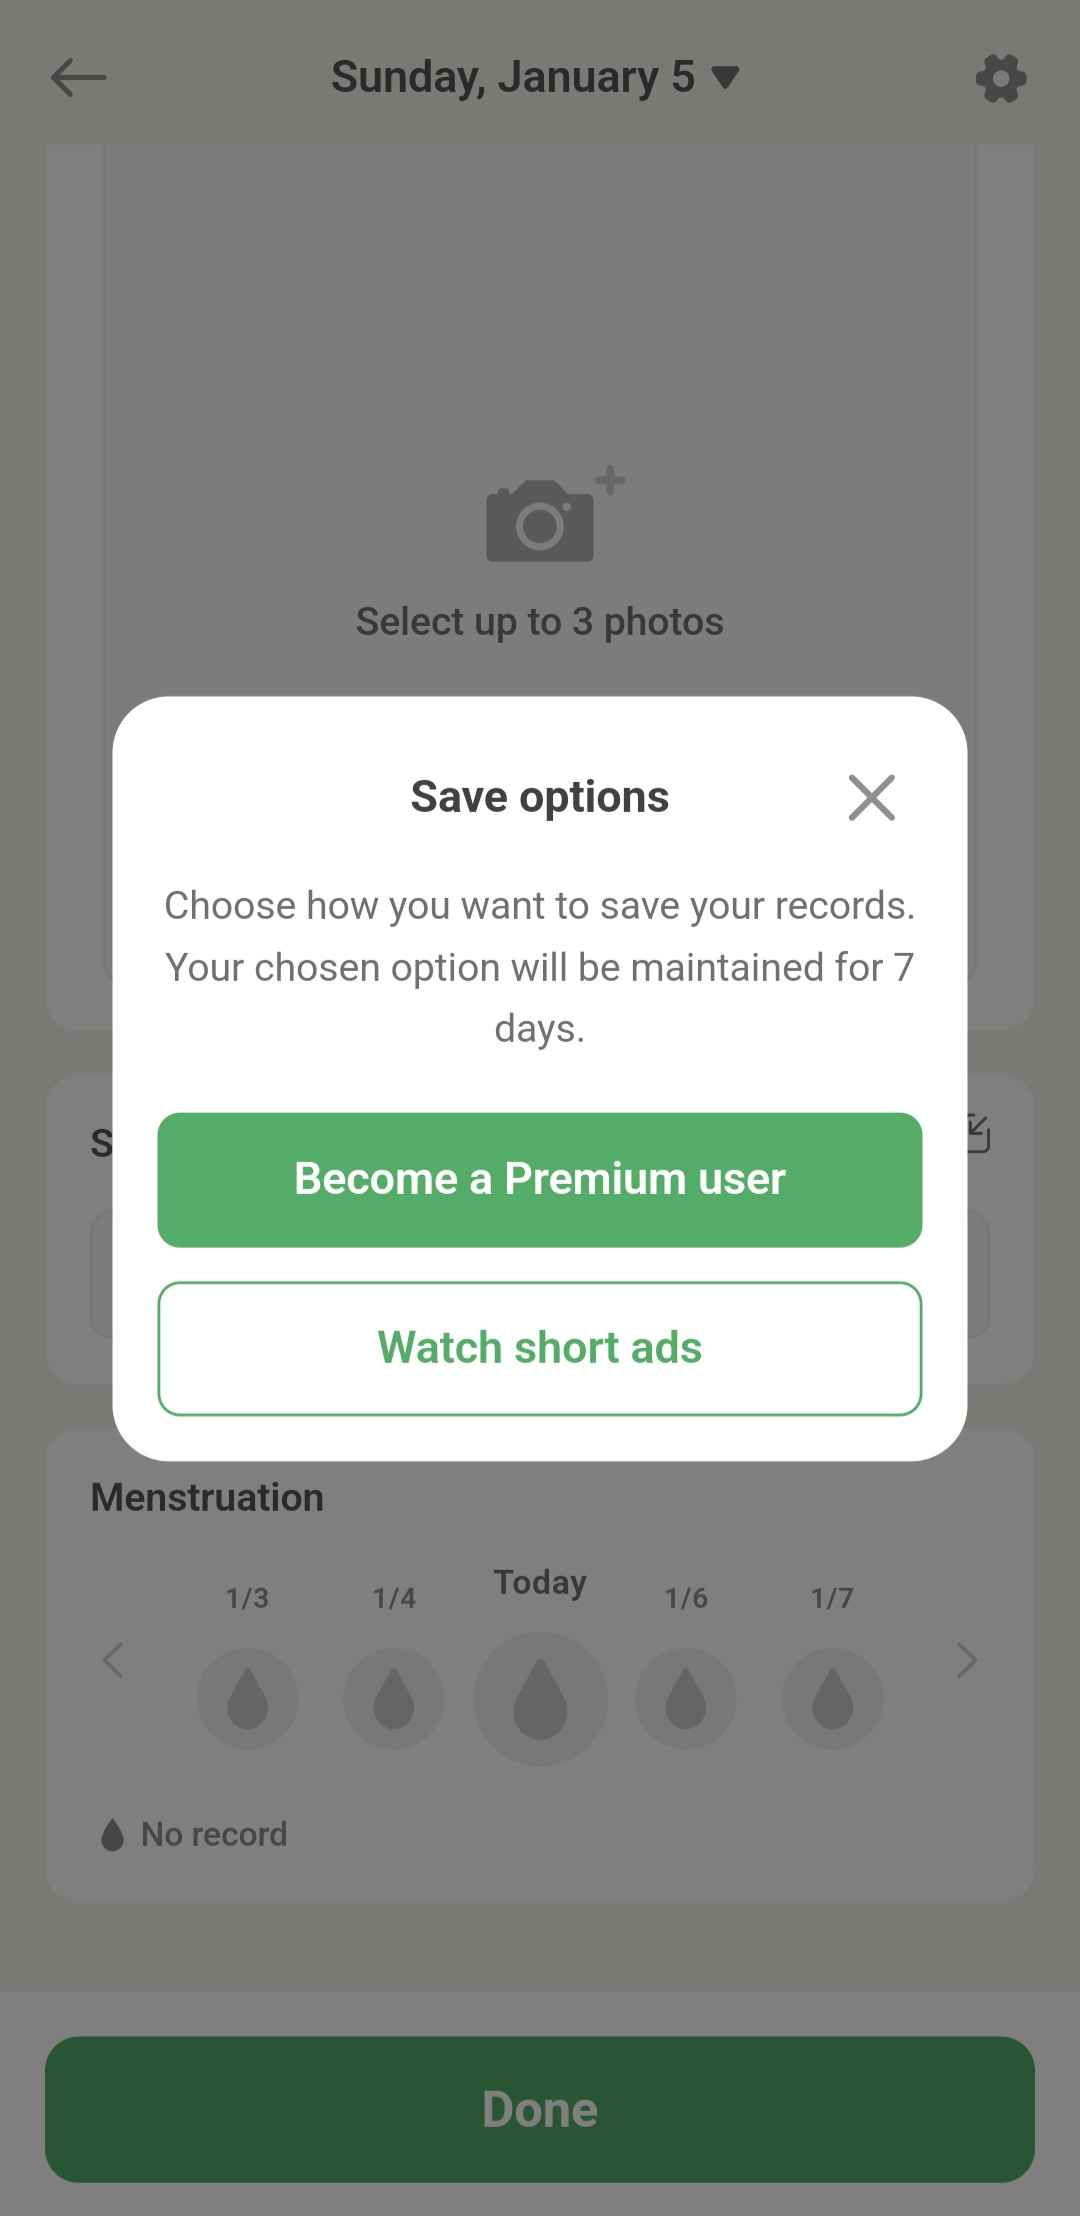
\includegraphics[width=0.35\textwidth]{dailybean3.jpg} 
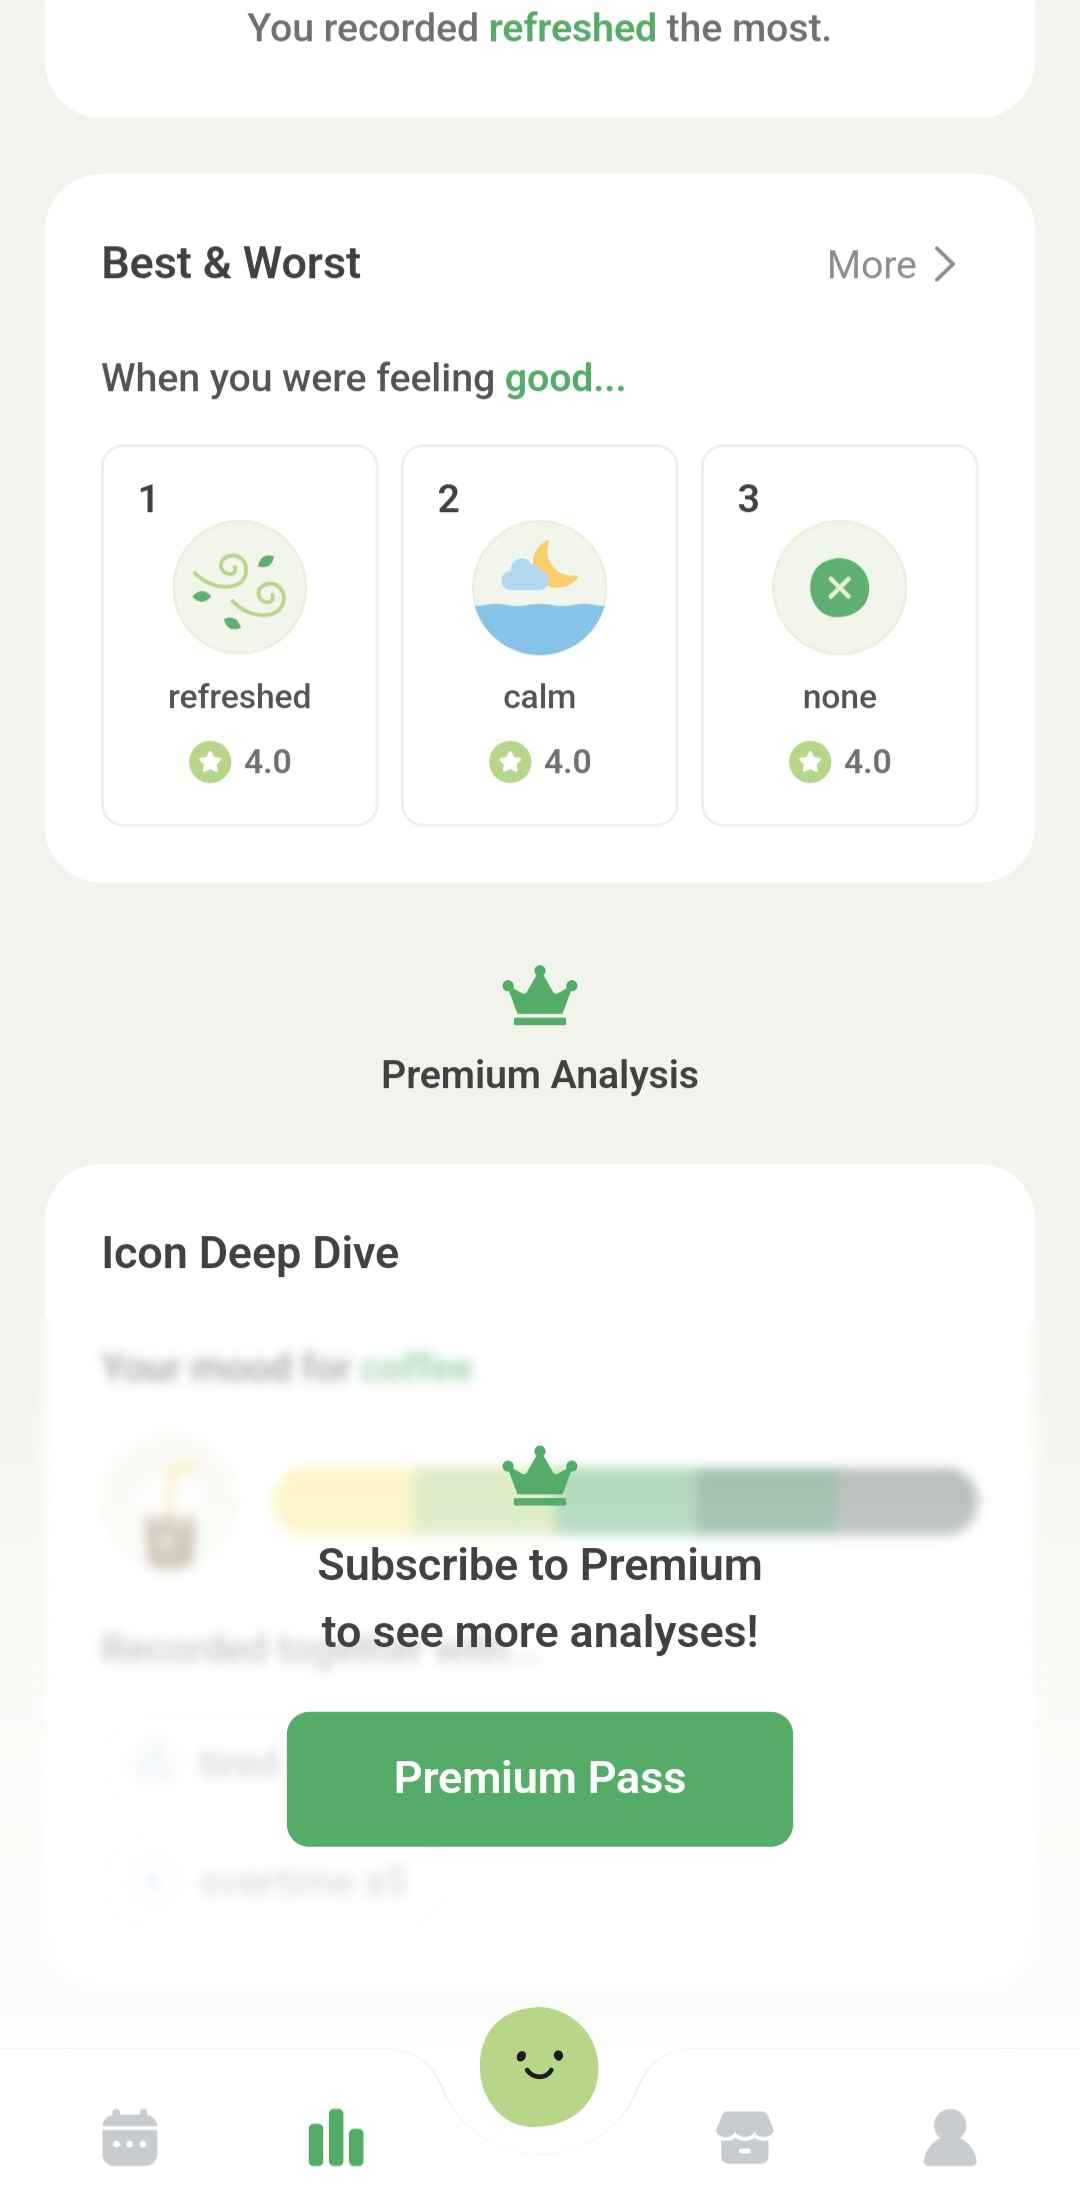
\includegraphics[width=0.35\textwidth]{dailybean5.jpg} 
\caption{Ograniczenia w bezpłatnej wersji aplikacji \textit{DailyBean}.}
\end{figure}

\section{How We Feel}
Ostatnią, i za razem najbardziej zbliżoną do naszego planowanego rozwiązania, aplikacją jest \textit{How We Feel}, stworzona z udziałem wspomnianego wcześniej Marca Bracketta. Korzystając z dwuwymiarowego modelu emocji, ta aplikacja pozwala użytkownikowi dogłębniej przeanalizować swój stan emocjonalny. \textit{How We Feel} jest zdecydowanie najdokładniejszą pod względem analizy psychologicznej z wszystkich porównanych dotąd aplikacji, natomiast posiada kilka drobnych wad. 

Ekran wyboru emocji (Rys 4.6) zapewnia dużą różnorodność, ale może przytłoczyć użytkownika ilością elementów. Nie ma też możliwości wyboru więcej niż jednej emocji, poza zaczynaniem procesu identyfikacji od początku, co wydaje się być potencjalnie uciążliwe dla osób chcących szybko i sprawnie zapisać swoje samopoczucie. 

Mimo tego, aplikacja wyróżnia się swoją bazą emocji, imponującym zestawem statystyk generowanych na podstawie historii wpisów użytkownika oraz estetycznym interfejsem, czyniąc ją jedną z naszych głównych inspiracji.

\begin{figure}[!t]
\centering
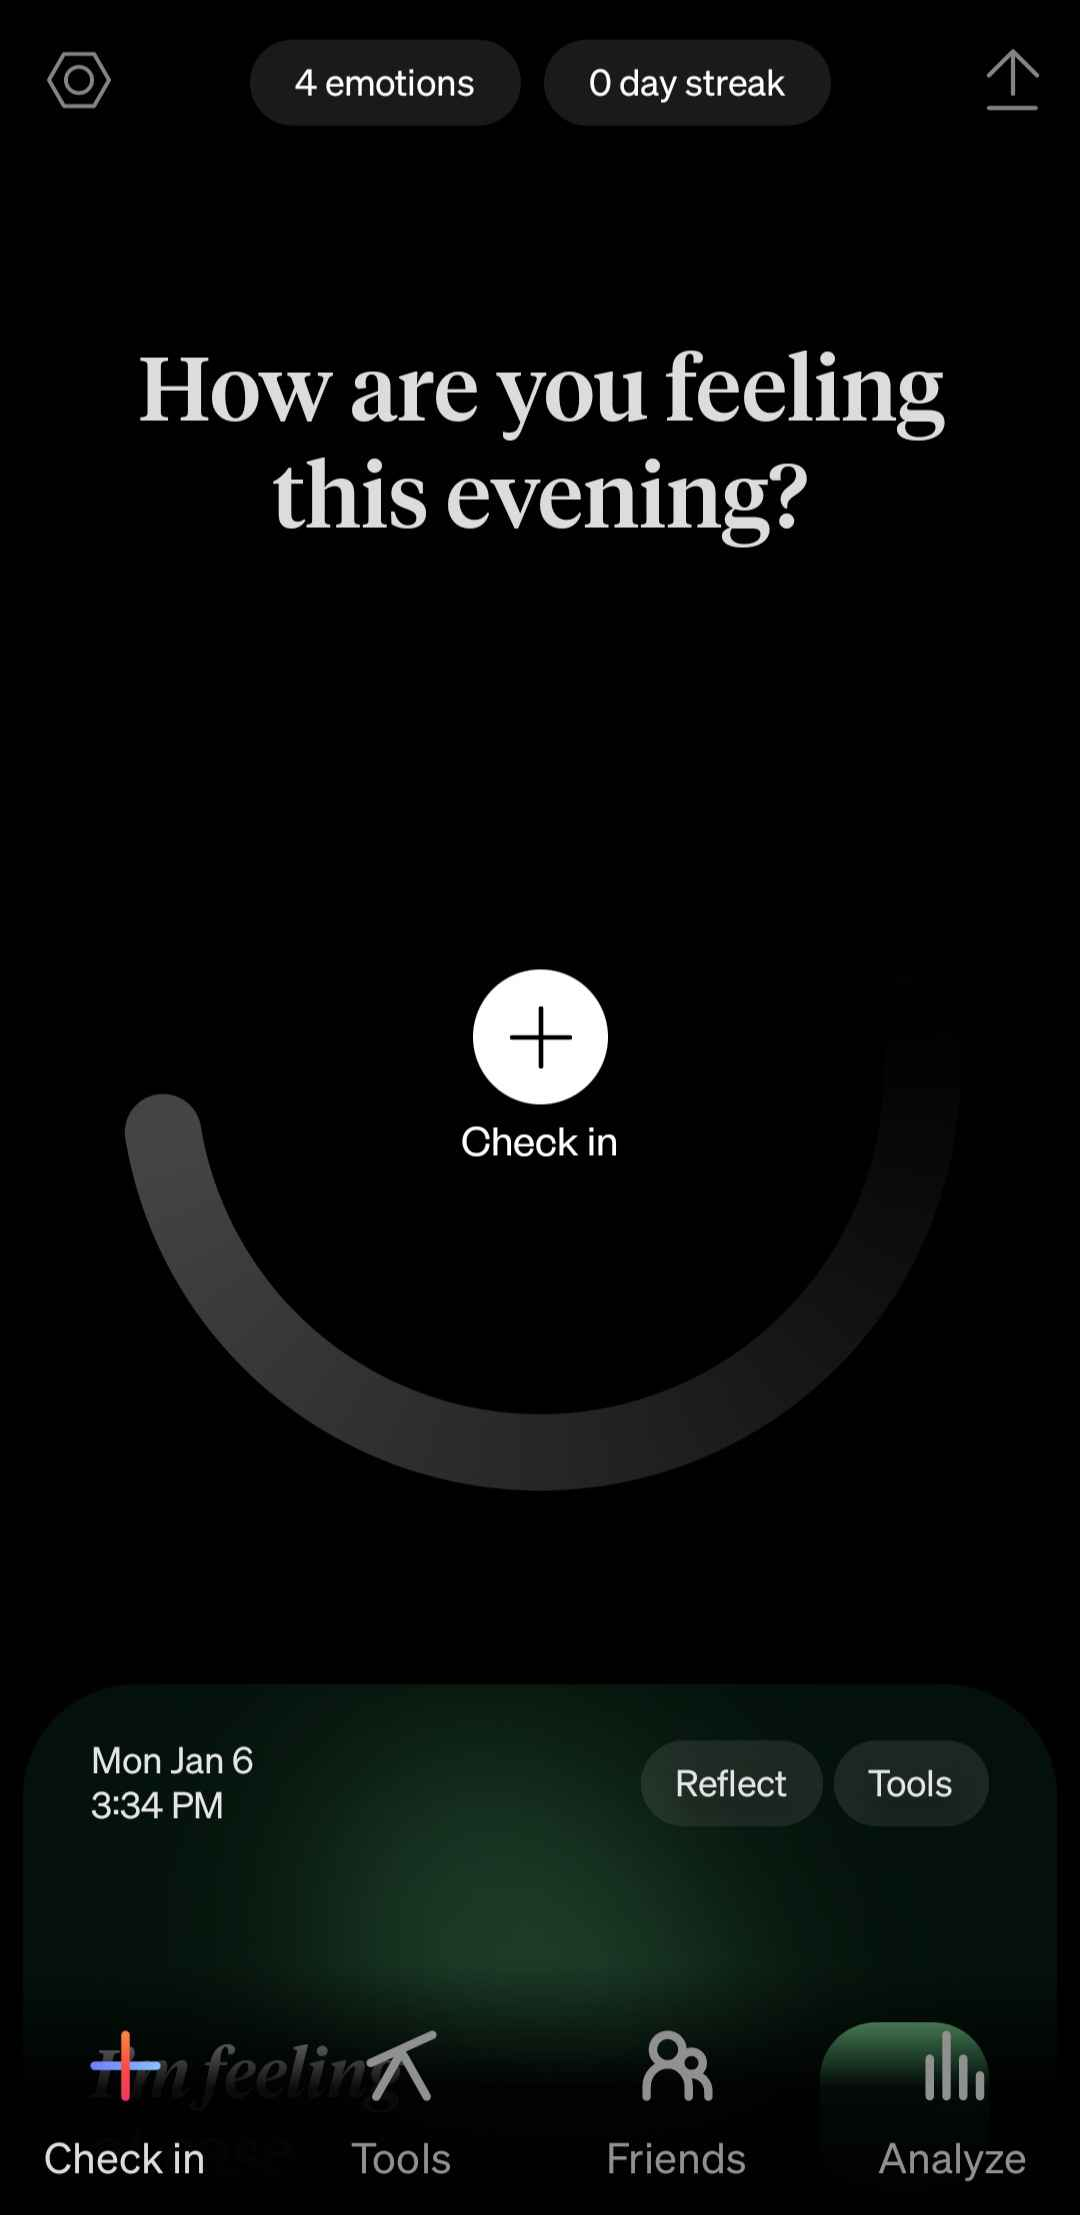
\includegraphics[width=0.3\textwidth]{howwefeel1.jpg} 
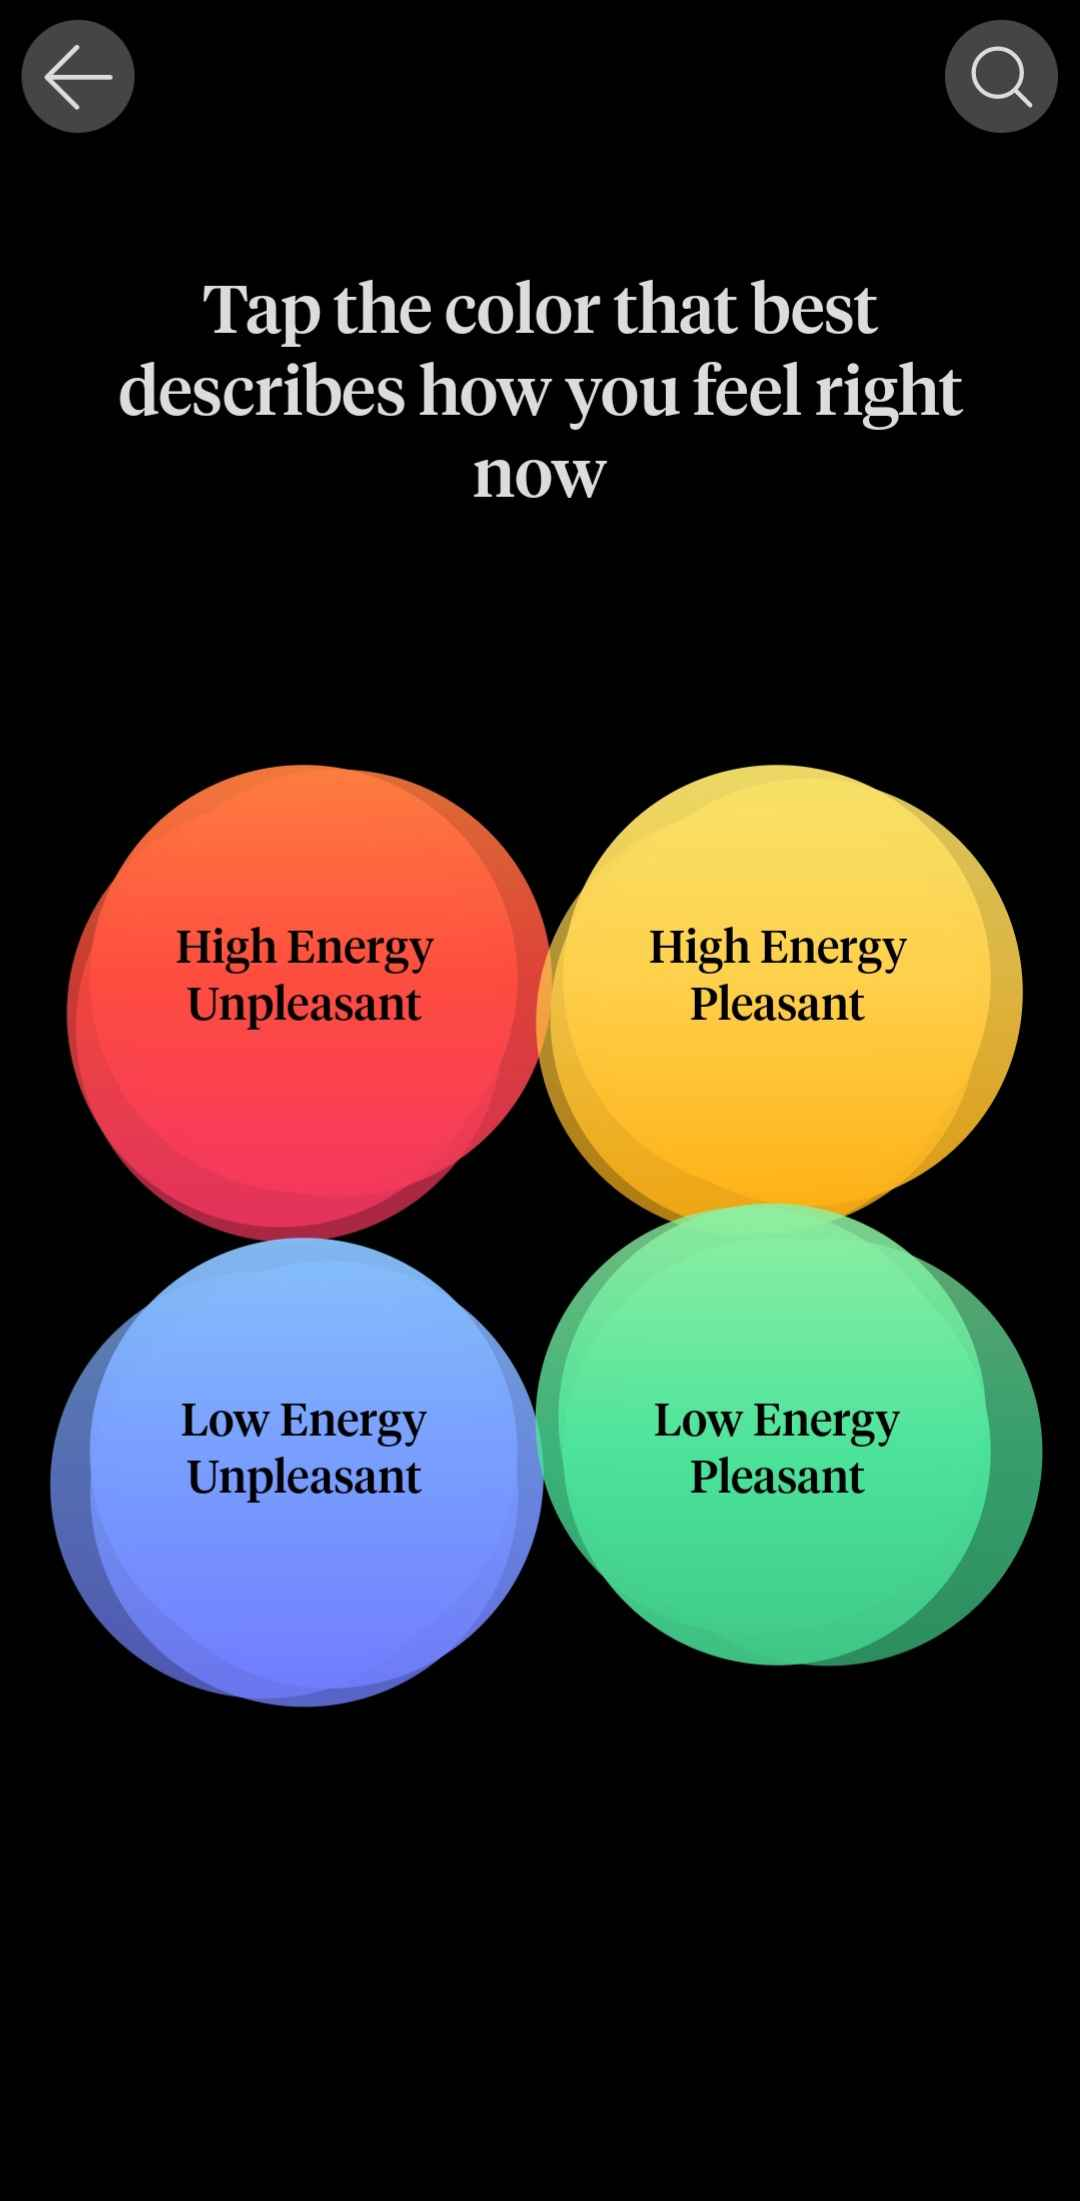
\includegraphics[width=0.3\textwidth]{howwefeel2.jpg} 
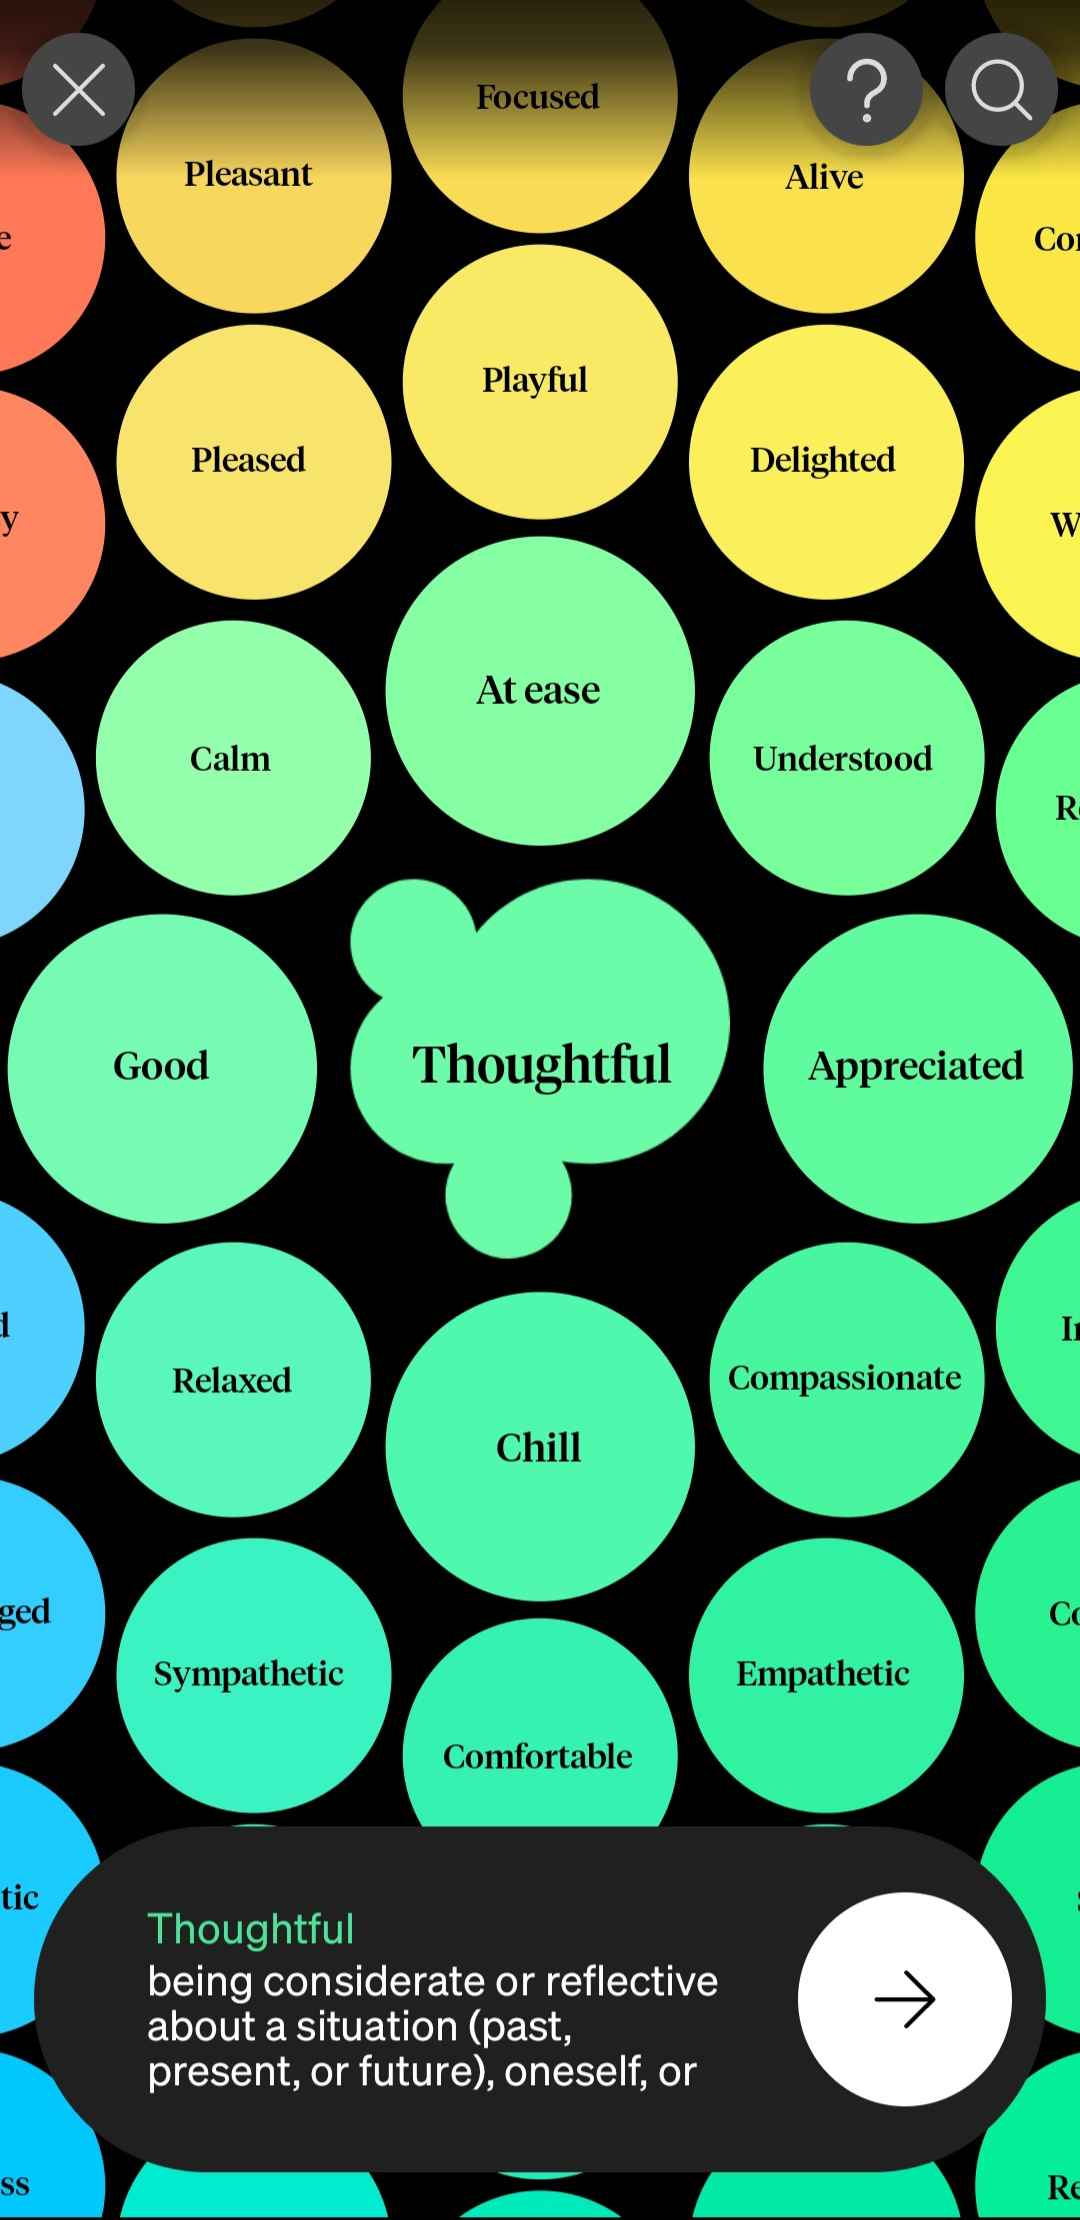
\includegraphics[width=0.3\textwidth]{howwefeel3.jpg} 
\caption{Widoki wybierania emocji w aplikacji \textit{How We Feel}.}
\end{figure}

\section{Wnioski}
Porównując dostępne na rynku aplikacje, miałyśmy okazję przyjrzeć się różnym pomysłom na narzędzia do analizy samopoczucia. Zmotywowało nas to do zwrócenia szczególnej uwagi na estetykę naszego interfejsu oraz skupieniu się na kilku dobrze dopracowanych funkcjonalnościach, aby zapewnić użytkownikowi płynne i przyjemne korzystanie z aplikacji.


\chapter{Wykaz narzędzi}
\section{Projekt interfejsu}

Do zaprojektowania interfejsu użyłyśmy platformy \textit{Figma}. Zaczęłyśmy od stworzenia prostego prototypu \textit{low fidelity}, aby mieć lepsze spojrzenie na układ widoków oraz strukturę aplikacji.

\begin{figure}[!h]
\centering
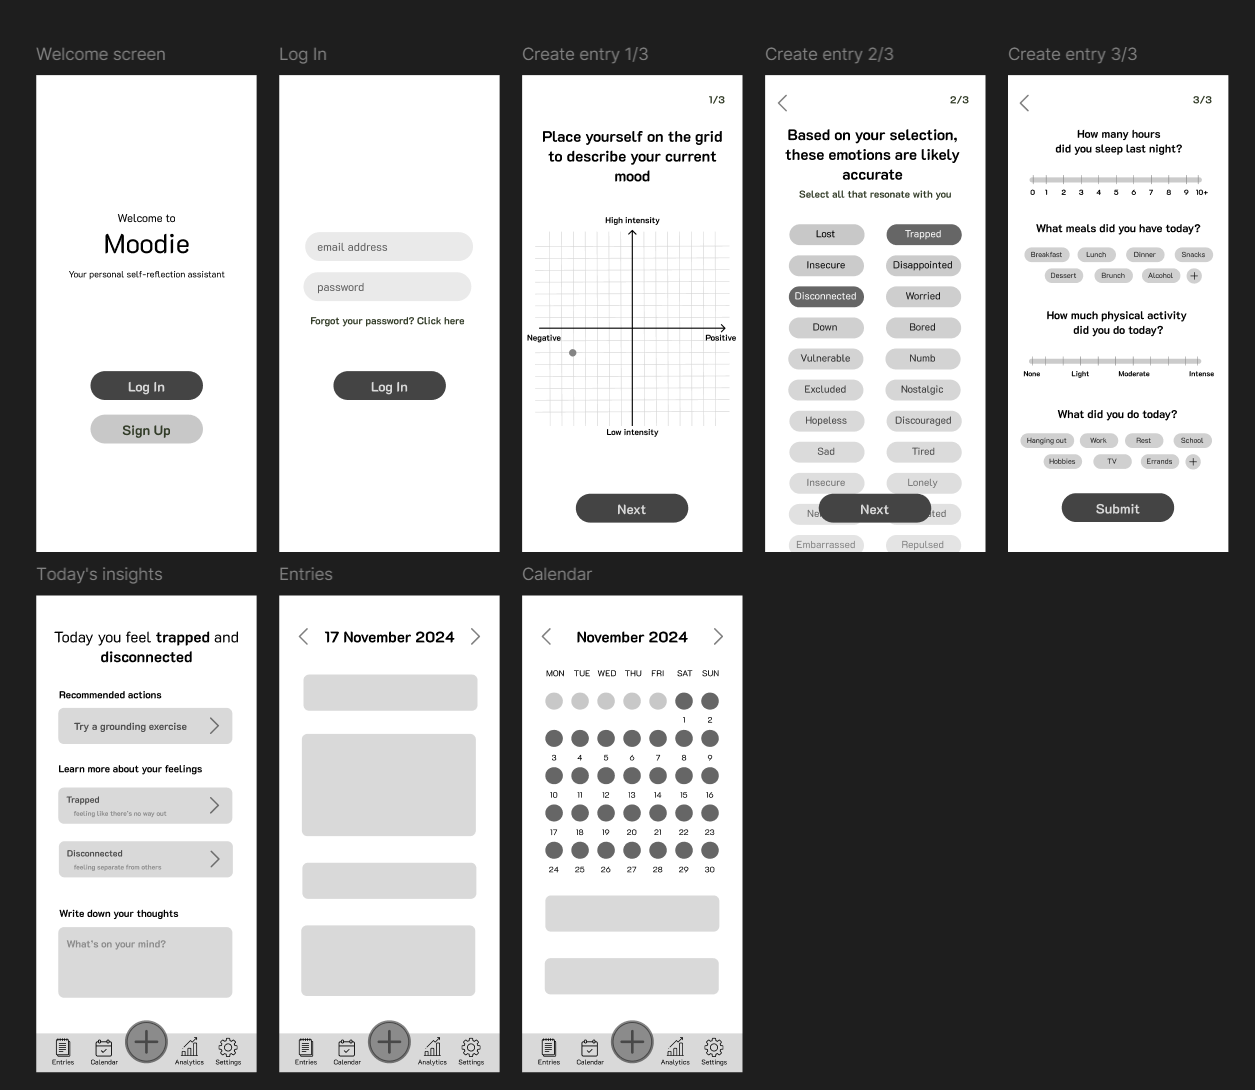
\includegraphics[width=0.95\textwidth]{figma-ui-lofi.png} 
\caption{Pierwszy prototyp interfejsu użytkownika.}
\end{figure}

Następnie na podstawie prototypu zaprojektowałyśmy faktyczny interfejs użytkownika gotowy do zaimplementowania. Naszym głównym celem było stworzenie spójnej gamy barw, kojarzącej się z wewnętrznym spokojem, przejrzystością i poczuciem równowagi.


\begin{figure}[!h]
\centering
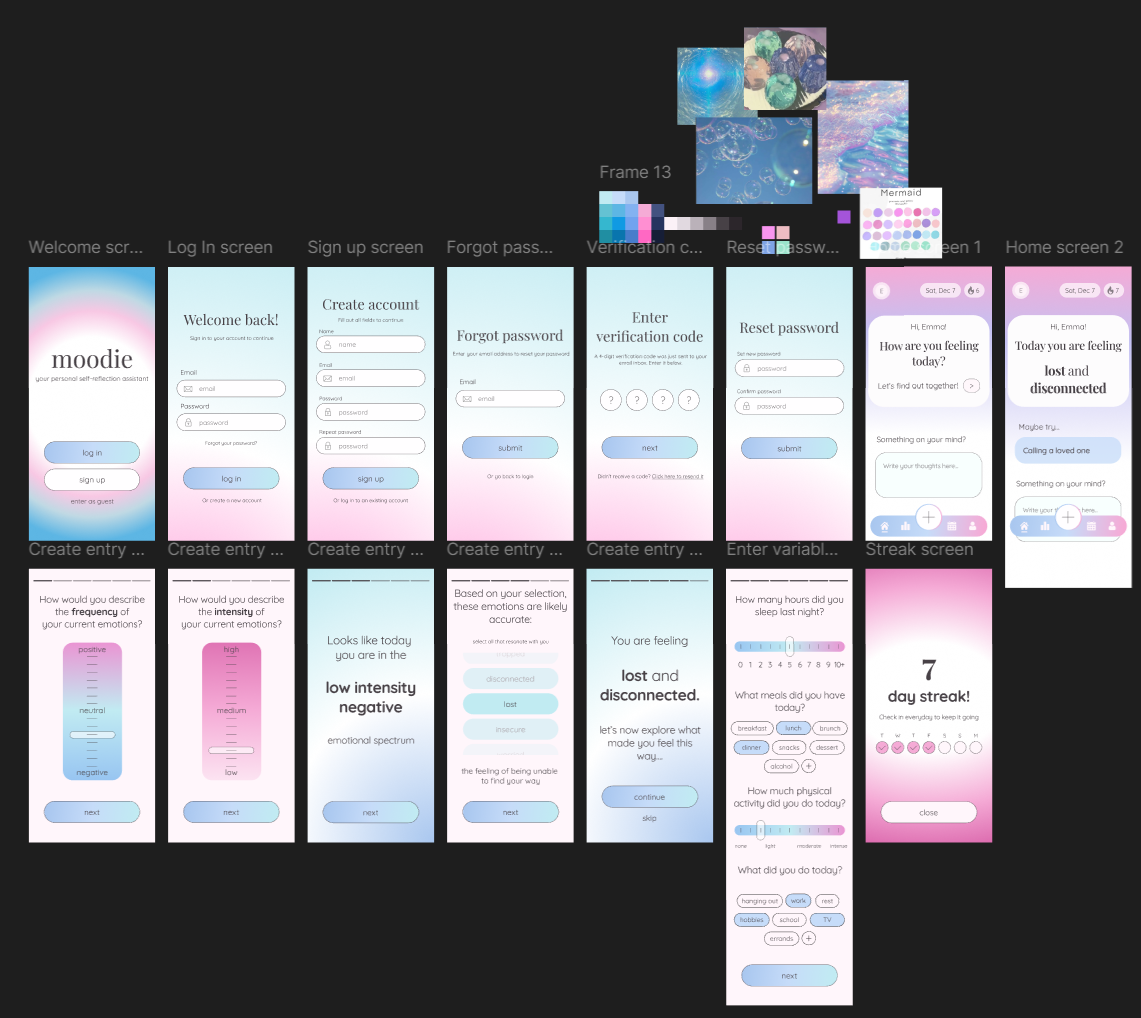
\includegraphics[width=0.9\textwidth]{figma-ui.png} 
\caption{Ostateczny projekt interfejsu użytkownika.}
\end{figure}

\section{Frontend}
Frontend aplikacji napisałyśmy w \textit{Javascript} za pomocą frameworka \textit{React Native} oraz \textit{Expo}. Do tworzenia zapytań HTTP komunikujących się z serwerem użyłyśmy biblioteki \textit{Axios}.

\section{Backend}
Serwer opracowałyśmy za pomocą \textit{Express.js}. Na początku trzymałyśmy go w tym samym repozytorium \textit{Git} co frontend, ale ostatecznie zdecydowałyśmy się na przeniesienie naszego backendu do osobnego repozytorium, aby ułatwić hostowanie go w chmurze. W celu wdrożenia kodu skorzystałyśmy z serwisu \textit{Render}.
\section{Baza danych}
Wybór odpowiedniego narzędzia do zarządzania bazą danych okazał się być dość problematycznym zagadnieniem. Początkowo założyłyśmy, że użyjemy \textit{SQLite} lub \textit{MongoDB} w zależności od tego, czy będzie nam potrzebna relacyjność bazy danych. Po większym rozeznaniu zdałyśmy sobie sprawę, że będziemy potrzebować serwisu, który bezpłatnie zaoferuje przetrzymywanie naszej bazy w chmurze. Jedną z najpopularniejszych takich platform jest \textit{Firebase}. Oferuje ona dodatkowo wiele gotowych narzędzi ułatwiających autentykację użytkownika czy analizę wydajności oprogramowania, jednak model danych opierający się na \textit{NoSQL} wydawał się niewystarczający na potrzeby naszej aplikacji. 

Ostatecznie udało nam się znaleźć \textit{Supabase}, alternatywne narzędzie oferujące podobne funkcjonalności, korzystające z obiektowo-relatywnej bazy danych \textit{PostgreSQL}. Ten wybór pozwolił nam zaoszczędzić czas na implementacji własnej logiki uwierzytelniania czy resetowania hasła i skupić się na ciekawszych elementach aplikacji.
\chapter{Podręcznik użytkownika}
\section{Instalacja}
\section{Przegląd aplikacji}

\ldots

\chapter{Podsumowanie}
Proces tworzenia naszej aplikacji był niezwykłym wyzwaniem, ale też idealną okazją do rozwoju. Byłyśmy odpowiedzialne za każde zagadnienie związane z urzeczywistnianiem naszego początkowego pomysłu oraz udoskonalaniem go w trakcie, co pokazało nam, z jak wielu czynników składa się budowanie aplikacji mobilnej. 

Niestety nie byłyśmy w stanie całkowicie sprostać naszym własnym oczekiwaniom. Miałyśmy w planach dodać o wiele więcej funkcjonalności, na które ostatecznie nie starczyło nam czasu lub zasobów. Jedną z nich było wyświetlanie personalizowanych wskazówek na podstawie emocji odczuwanych przez użytkownika danego dnia. Wskazówki te miały brać też pod uwagę kontekst dotyczący snu, aktywności fizycznej itp. i odpowiednio proponować pewne czynności (np. \textit{zadzwoń do kogoś bliskiego}, \textit{pojdź na spacer} czy \textit{posłuchaj swojej ulubionej piosenki}), ale zdałyśmy sobie sprawę, że do zbudowania na tyle zniuansowanej bazy potrzebowałybyśmy pomocy licencjonowanego specjalisty czy psychologa. 

Nie udało nam się też pokryć naszego kodu testami jednostkowymi i integracyjnymi. W przypadku dalszego rozwoju aplikacji, byłoby to jednym z ważniejszych zadań do nadrobienia. Dzięki temu znacznie usprawniłby się proces modyfikowania istniejących funkcji oraz znajdowania błędów w kodzie. W przyszłości chciałybyśmy też dodać możliwość zmiany języka aplikacji, aby rozszerzyć grono potencjalnych odbiorców.

Mimo wszystko, jesteśmy zadowolone z efektu końcowego naszej aplikacji. Udało nam się zaprojektować rozwiązanie, które ma potencjał istotnie przyczynić się do poprawy jakości życia użytkowników.

%%%%% BIBLIOGRAFIA

\begin{thebibliography}{1}

\bibitem{} Marc Brackett, \textit{Permission To Feel}

Link: https://marcbrackett.com/permission-to-feel/

\bibitem{} Jody Michael Associates, \textit{Feelings, Emotions and Moods: How to Say What You are Experiencing}

Link: https://www.jodymichael.com/blog/jma-feelings-list/

\bibitem{} Berkeley Well-Being Institute, \textit{List of Emotions: 271 Emotion Words}

Link: https://www.berkeleywellbeing.com/list-of-emotions.html

\bibitem{} James A. Russel, \textit{A Circumplex Model of Affect (1980)}

Link: https://www.researchgate.net/publication/235361517\_A\_Circumplex\_Model\_of\_Affect

\bibitem{} How We Feel

Link: https://howwefeel.org

\bibitem{} React Native

Link: https://reactnative.dev
\bibitem{} Expo

Link: https://expo.dev

\bibitem{} Express.js

Link: https://expressjs.com

\bibitem{} Supabase

Link: https://supabase.com

\bibitem{} Render 

Link: https://render.com

\bibitem{} PostgreSQL

Link: https://www.postgresql.org.pl

\bibitem{} Figma

Link: https://www.figma.com

\end{thebibliography}

\end{document}
